\documentclass[10pt,twocolumn,letterpaper]{article}

\usepackage{cvpr}
\usepackage{times}
\usepackage{epsfig}
\usepackage{graphicx}
\usepackage{amsmath}
\usepackage{amssymb}

% Include other packages here, before hyperref.
\usepackage{algorithm}
\usepackage{algpseudocode}
\usepackage{wrapfig}
\usepackage{subcaption}

\usepackage{caption}
\captionsetup[table]{position=bottom}

\usepackage{array}
\usepackage{epstopdf}
\usepackage{cuted}

% If you comment hyperref and then uncomment it, you should delete
% egpaper.aux before re-running latex.  (Or just hit 'q' on the first latex
% run, let it finish, and you should be clear).
\usepackage[pagebackref=true,breaklinks=true,letterpaper=true,colorlinks,bookmarks=false]{hyperref}

% \cvprfinalcopy % *** Uncomment this line for the final submission

\def\cvprPaperID{3722} % *** Enter the CVPR Paper ID here
\def\httilde{\mbox{\tt\raisebox{-.5ex}{\symbol{126}}}}

% Pages are numbered in submission mode, and unnumbered in camera-ready
\ifcvprfinal\pagestyle{empty}\fi

\begingroup
  \catcode`\_=\active
  \gdef_#1{\ensuremath{\sb{\mathrm{#1}}}}
\endgroup
\mathcode`\_=\string"8000
\catcode`\_=12

\usepackage{xcolor}
\usepackage{textcomp}
\definecolor{Gray}{rgb}{0.5,0.5,0.5}
\definecolor{darkblue}{rgb}{0,0,0.7}
\definecolor{orange}{rgb}{1,.5,0} % something readable but different from todo
\definecolor{red}{rgb}{1,0,0} % something readable but different from todo
\newcommand{\heading}[1]{\noindent\textbf{#1}}
\newcommand{\note}[1]{{\em{\textcolor{orange}{#1}}}}
\newcommand{\todo}[1]{{\textcolor{darkblue}{TODO: #1}}}
\newcommand{\changed}[1]{{\textcolor{blue}{#1}}}

\newcommand{\Matrix}[1]     {{\ensuremath{\mathbf{\uppercase{#1}}}}} %Matrix 
\newcommand{\Vector}[1]     {{\ensuremath{\mathbf{\lowercase{#1}}}}} %Vector
\newcommand{\Variable}[1]   {{\ensuremath{\mathrm{\lowercase{#1}}}}} %Scalar
\newcommand{\Id}            {\mathbb{I}} %Identity matrix

\newcommand{\mini}[1]   {\underset{{#1}}{\operatorname{min}} \: \: } %Minimize w.r.t.
\newcommand{\minimize}[1]   {\underset{{#1}}{\operatorname{argmin}} \: \: } %Minimize w.r.t.
\newcommand{\subjectto}     {\operatorname{subject to}}

\newcommand{\signal} {\Vector{x}}
\newcommand{\filter} {\Vector{d}}
\newcommand{\code}   {\Vector{z}}
\newcommand{\Filter} {\Matrix{D}}
\newcommand{\mask}   {\Matrix{M}}
\newcommand{\Code}   {\Matrix{z}}
\newcommand{\surC}   {\Matrix{C}}
\newcommand{\surB}   {\Matrix{B}}
\newcommand{\matA}   {\Matrix{A}}
\newcommand{\ite}	 {t}

\begin{document}

%%%%%%%%% TITLE
\title{Stochastic Convolutional Sparse Coding \\ Supplementary Material}

\author{First Author\\
Institution1\\
Institution1 address\\
{\tt\small firstauthor@i1.org}
% For a paper whose authors are all at the same institution,
% omit the following lines up until the closing ``}''.
% Additional authors and addresses can be added with ``\and'',
% just like the second author.
% To save space, use either the email address or home page, not both
\and
Second Author\\
Institution2\\
First line of institution2 address\\
{\tt\small secondauthor@i2.org}
}

\maketitle

\section{Solvers for LASSO and QCQP}
Algorithm~\ref{algo:ADMMLasso} is used to optimize a LASSO problem in the following form:
\begin{equation}
    \minimize{\code} \frac{1}{2}\|\signal - \Filter \code \|_2^2 + \lambda\| \code \|_1
\end{equation}

\begin{algorithm}
\caption{ADMM framework for solving LASSO} \label{algo:ADMMLasso}
\begin{algorithmic}[1]
    \For{$s=1$ to $S$}
        \State // z-update step (quadratic programming)
        \State $\code^{s+1} \gets (\Filter ^ \top \Filter + \rho \Id )^{-1}(\Filter^\top \signal + \rho(\Vector{y}^s - \Vector{q}^s ) )$
        \State // y-update step (soft thresholding)
        \State $\Vector{y}^{s+1} \gets (\code^{s+1}+\Vector{q}^{s} - \frac{\lambda}{\rho})_{+} ~ - ~ (-\code^{s+1}-\Vector{q}^{s} - \frac{\lambda}{\rho})_{+}$
        \State // scaled dual variables update
        \State $\Vector{q}^{s+1} \gets \bold{q}^{s}+\code^{s+1}-\Vector{y}^{s+1}$
    \EndFor
\end{algorithmic}
\end{algorithm}
$S$ is the total number of ADMM iteration. $\Vector{y}$ is the introduced slack variable, $\Vector{q}$ is the scaled dual variable, and $\rho$ is the augmented Lagrangian penalty.

\begin{algorithm}
\caption{Projected Block Coordinate Descent for solving QCQP} \label{algo:BCDQCQP}
\begin{algorithmic}[1]
\State $\Vector{r} \gets \signal - \Code \filter $
\While {not converge}
    \For{$k=1$ to $K$}
        \State $ \filter^{\ast}_k \gets \filter_k + \Code_k ^ \top \Vector{r} ~ / ~ L_k $
        \State $ \filter^{\ast}_k \gets \filter^{\ast}_k ~ / ~ \text{max}( \|\filter^{\ast}_k\|,1 ) $
        \State $ \Vector{r} ~~ \gets \Vector{r} + \Code_k( \filter_k - \filter^{\ast}_k ) $
    \EndFor
    \State  $ \filter \gets \filter^{\ast} $
\EndWhile
\end{algorithmic}
\end{algorithm}


Algorithm~\ref{algo:BCDQCQP} is used to optimize a QCQP problem in the following form:
\begin{equation}
\begin{split}
    \minimize{\filter} & \frac{1}{2}\|\signal - \Code \filter \|_2^2 \\
    \text{subject to} & ~ \|\filter_k\|^2_2 \leq 1 ~~ \forall k \in \{1,\dots,K\},
\end{split}
\end{equation}

$L_k$ is the Lipschitz constant of $\Code_k^\top \Code_k$.

\begin{figure*}[h]
\centering
\begin{subfigure}{0.49\textwidth}
  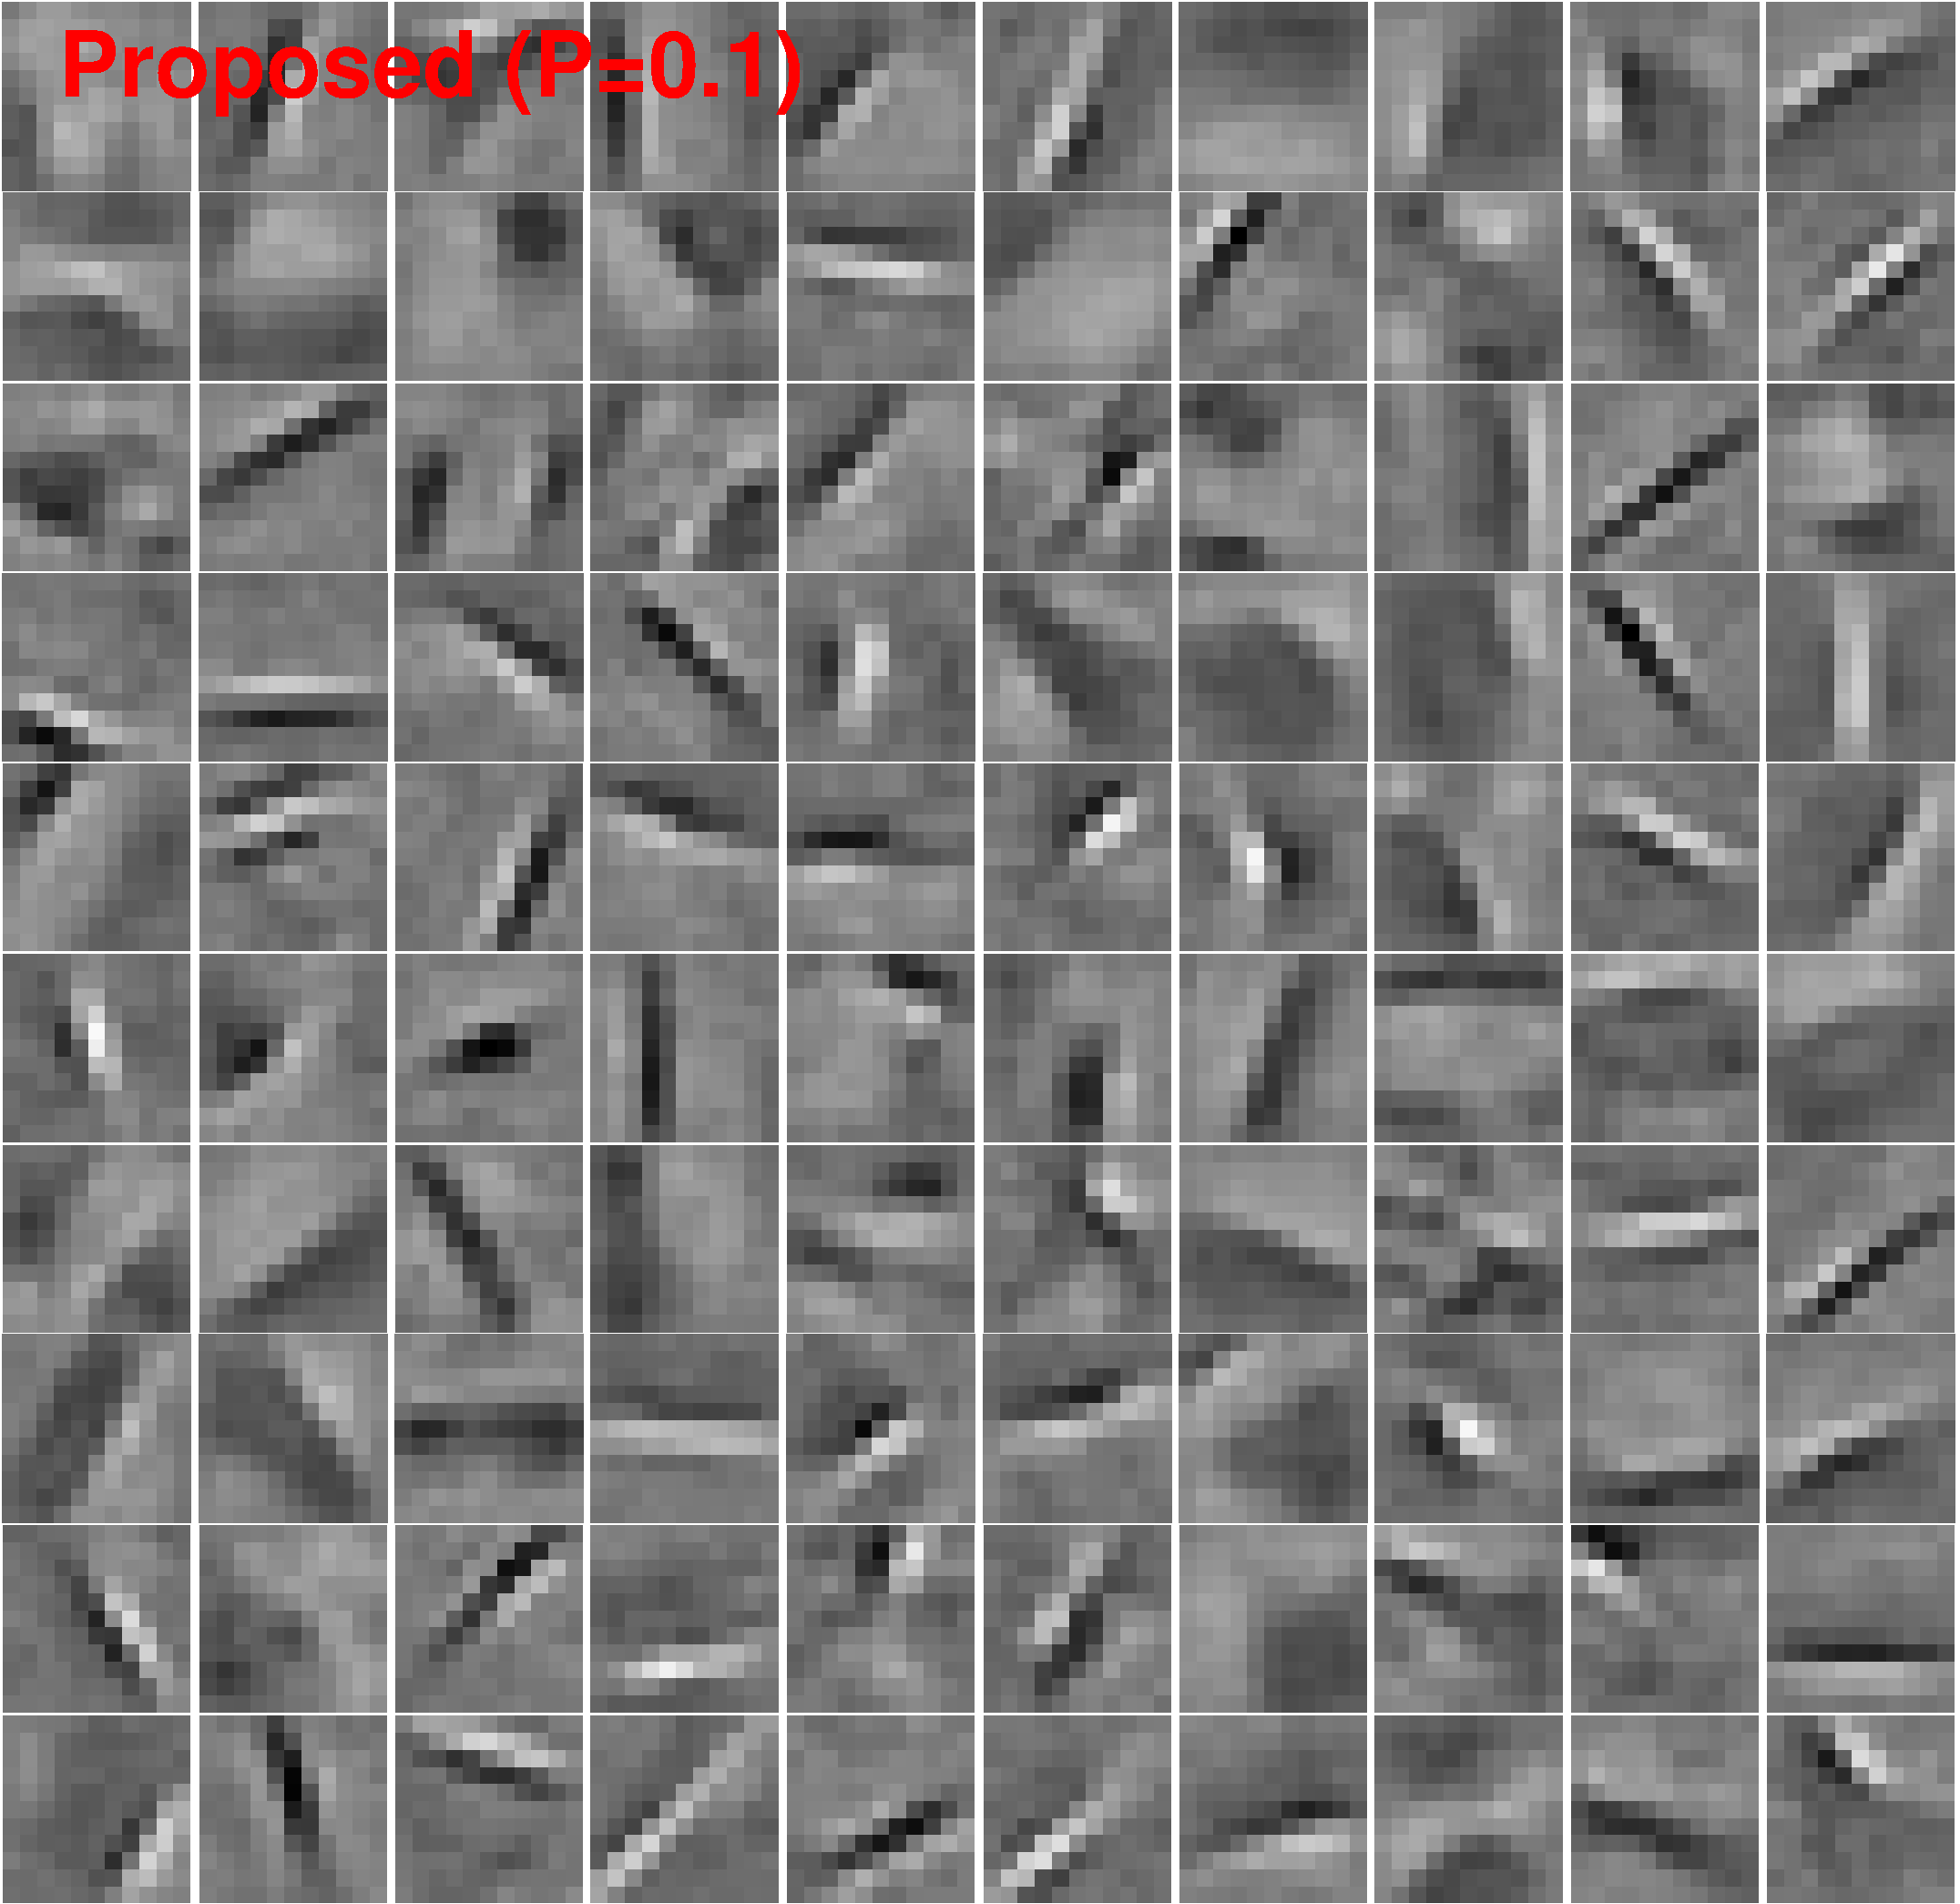
\includegraphics[width=1\linewidth]{figure/batchFruit100.pdf}
\end{subfigure}
\begin{subfigure}{0.49\textwidth}
  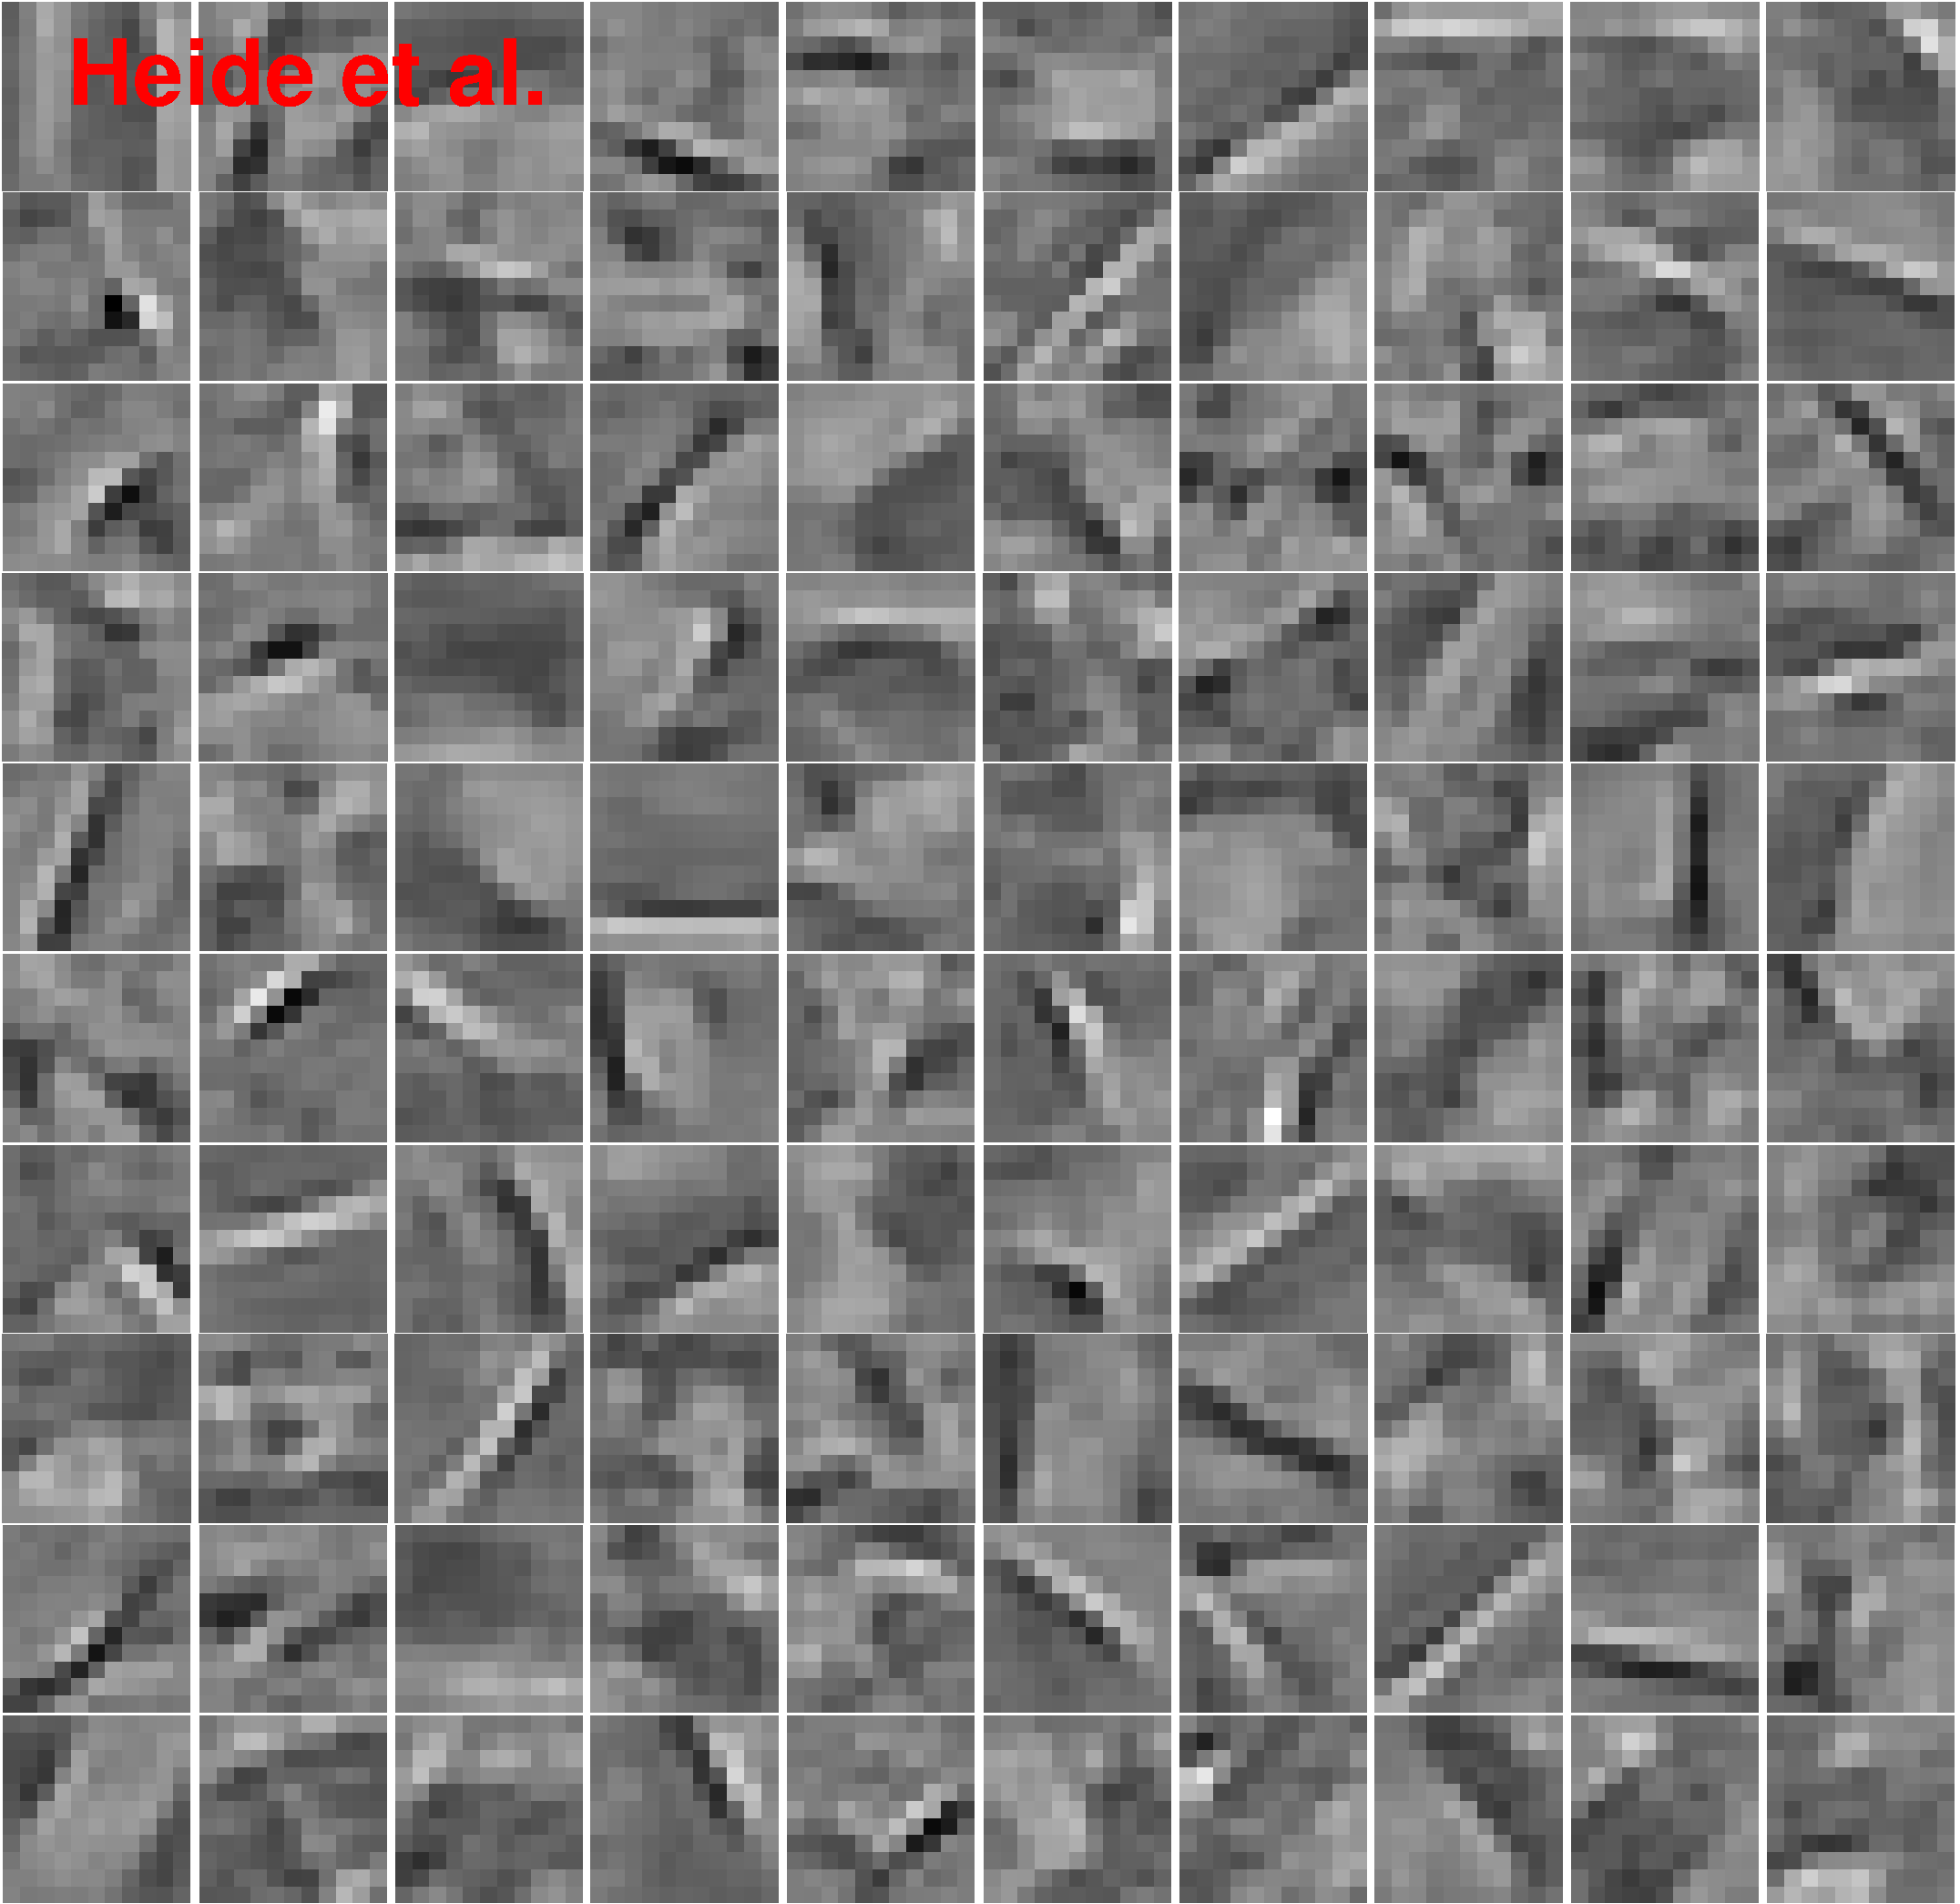
\includegraphics[width=1\linewidth]{figure/heideFruit100.pdf}
  \end{subfigure}
\caption{Zoom-in view of the filters from Fig.~1 of the main manuscript.}
\end{figure*}

\section{Zooming in on the Filters}

Here we zoom in on the filters from Fig.~1 in the main manuscript. Notice that our filters look more smooth for those Gabor-like filters and also contains less number of noise-like filters.

\section{Additional Experiments}
In order to show the robustness of the proposed algorithms, We also conduct experiments on city dataset. We first compare SBCSC with the state-of-the-art batch-mode algorithm, and the results are shown in Fig.\ \ref{fig:subsampleResult-city}. Similar to the results shown in Fig.~1 in the main manuscript, SBCSC, with $p=0.1$, outperforms the compared batch-mode algorithm with better outcomes and runtime performance. Since the learning is performed on handful datasets, both of them learn quite a few data-specific image features. These data-specific image features have the shortage of the generalization ability, which can be revealed in the image inpainting application. For example, the eighth image, which contains a large portion of the texture information existed in the filters learned from city dataset, can be significantly better reconstructed by such filters compared to using those learned from fruit dataset. However, it may exhibit poorer performance on other types of images. 

\begin{figure*}[h]
\begin{subfigure}{0.5\textwidth}
  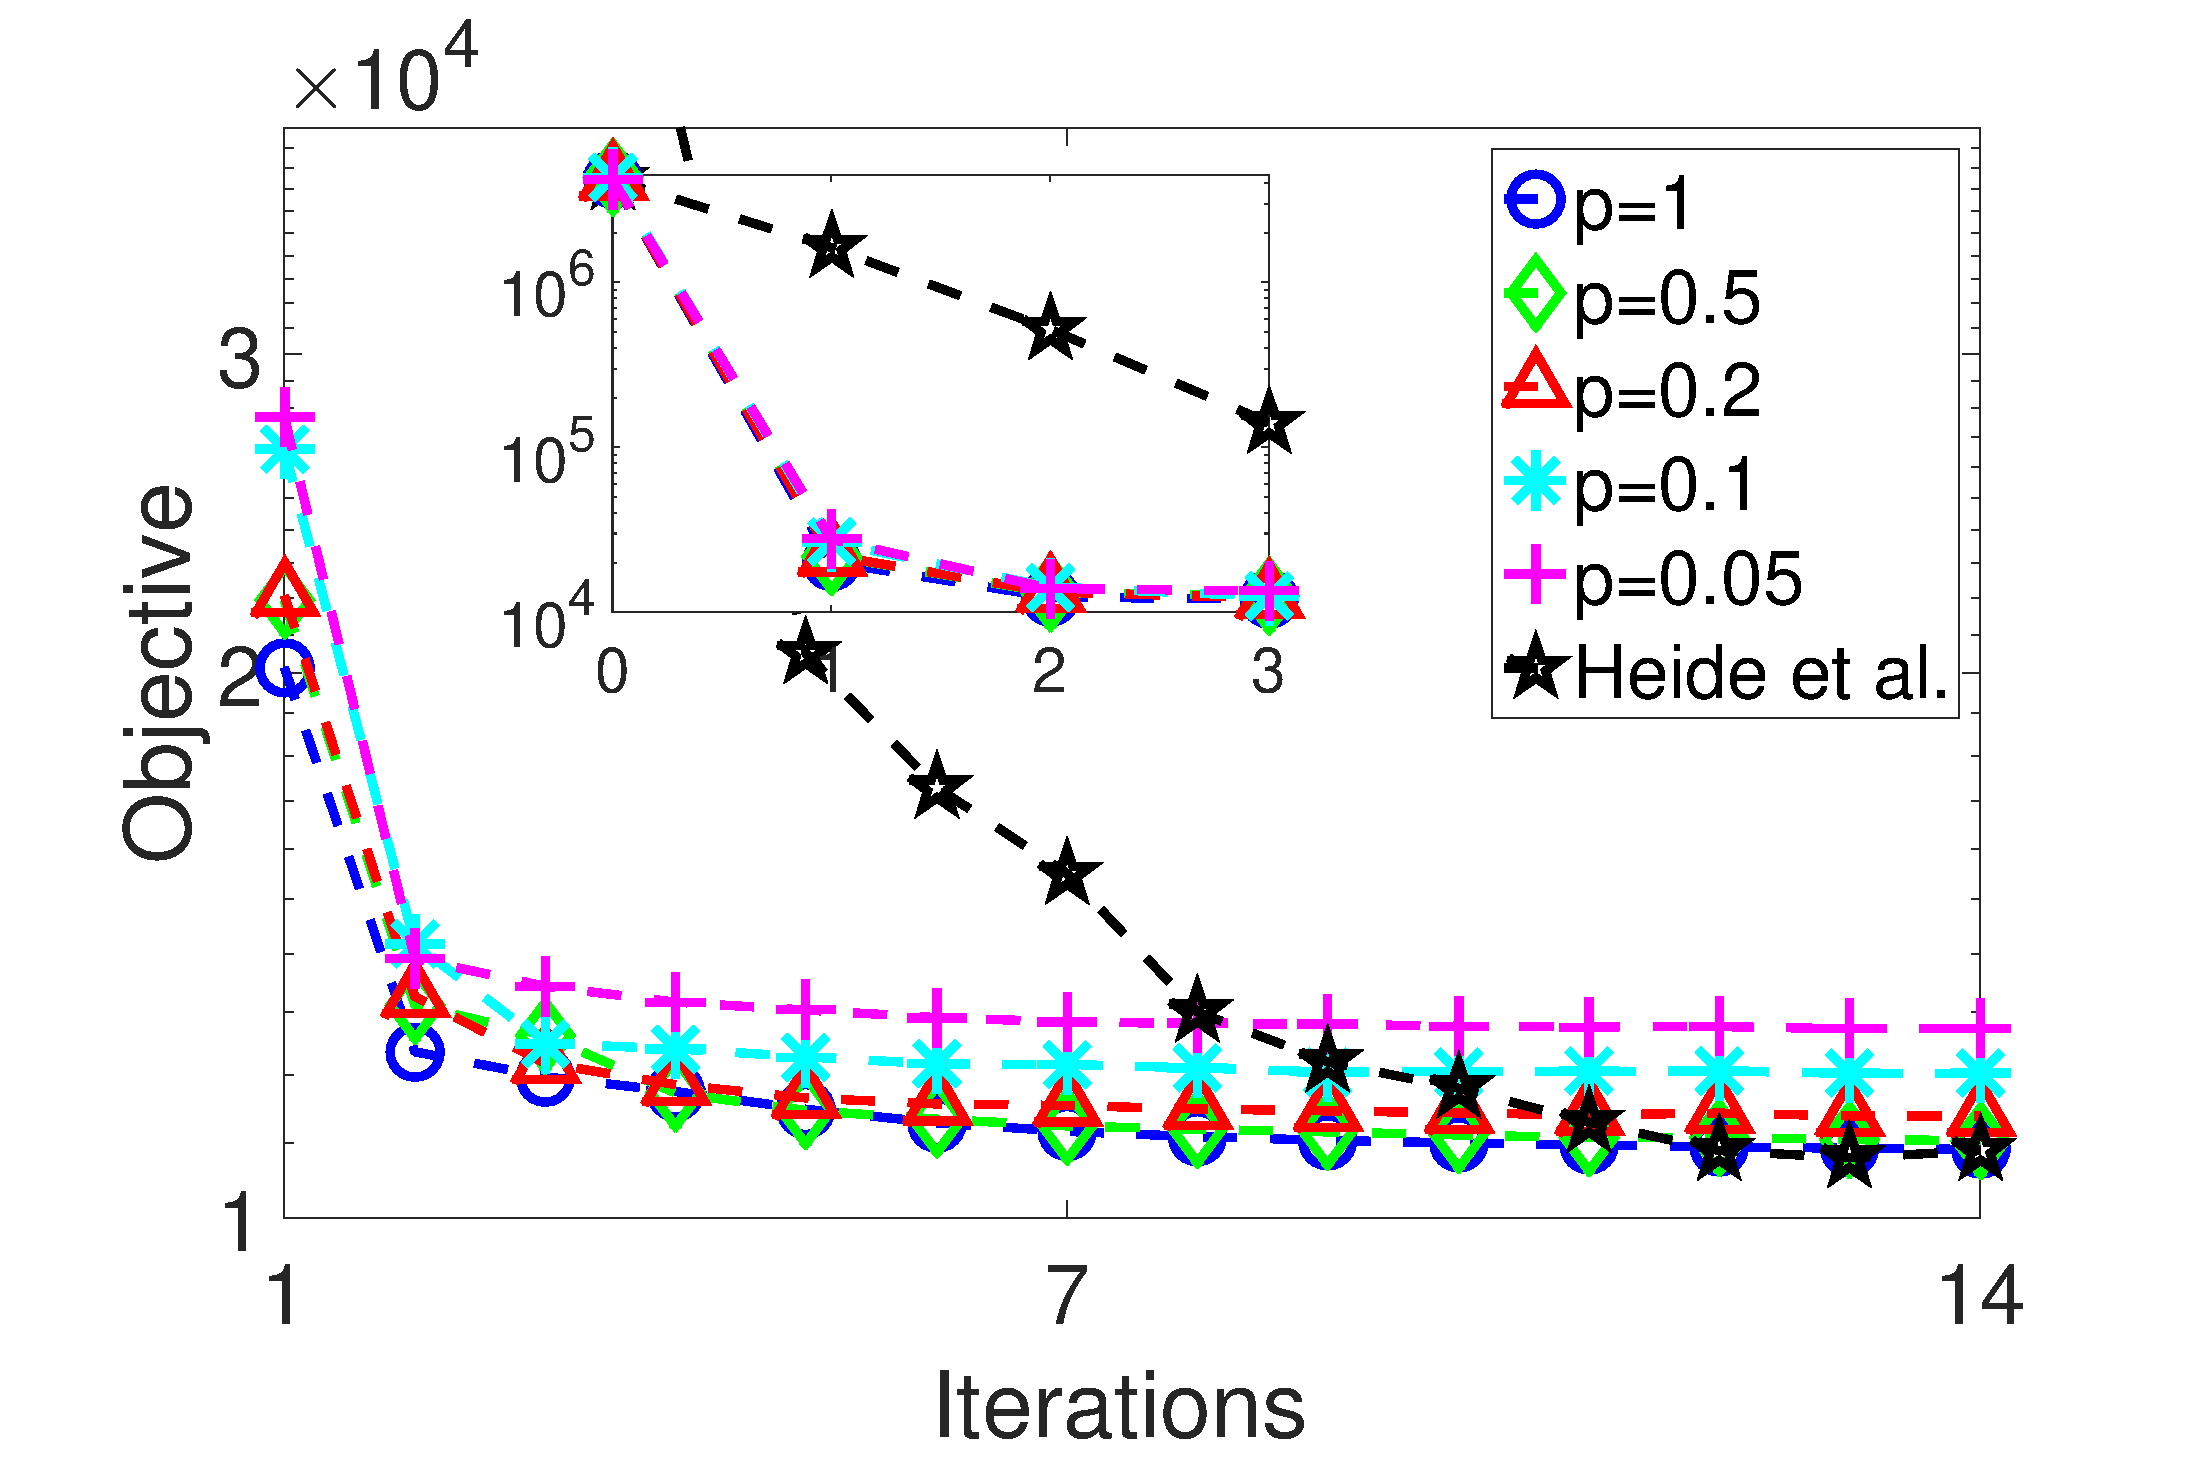
\includegraphics[width=1\linewidth]{figure/iteVSobj-city.pdf}
\end{subfigure}
\begin{subfigure}{0.5\textwidth}
  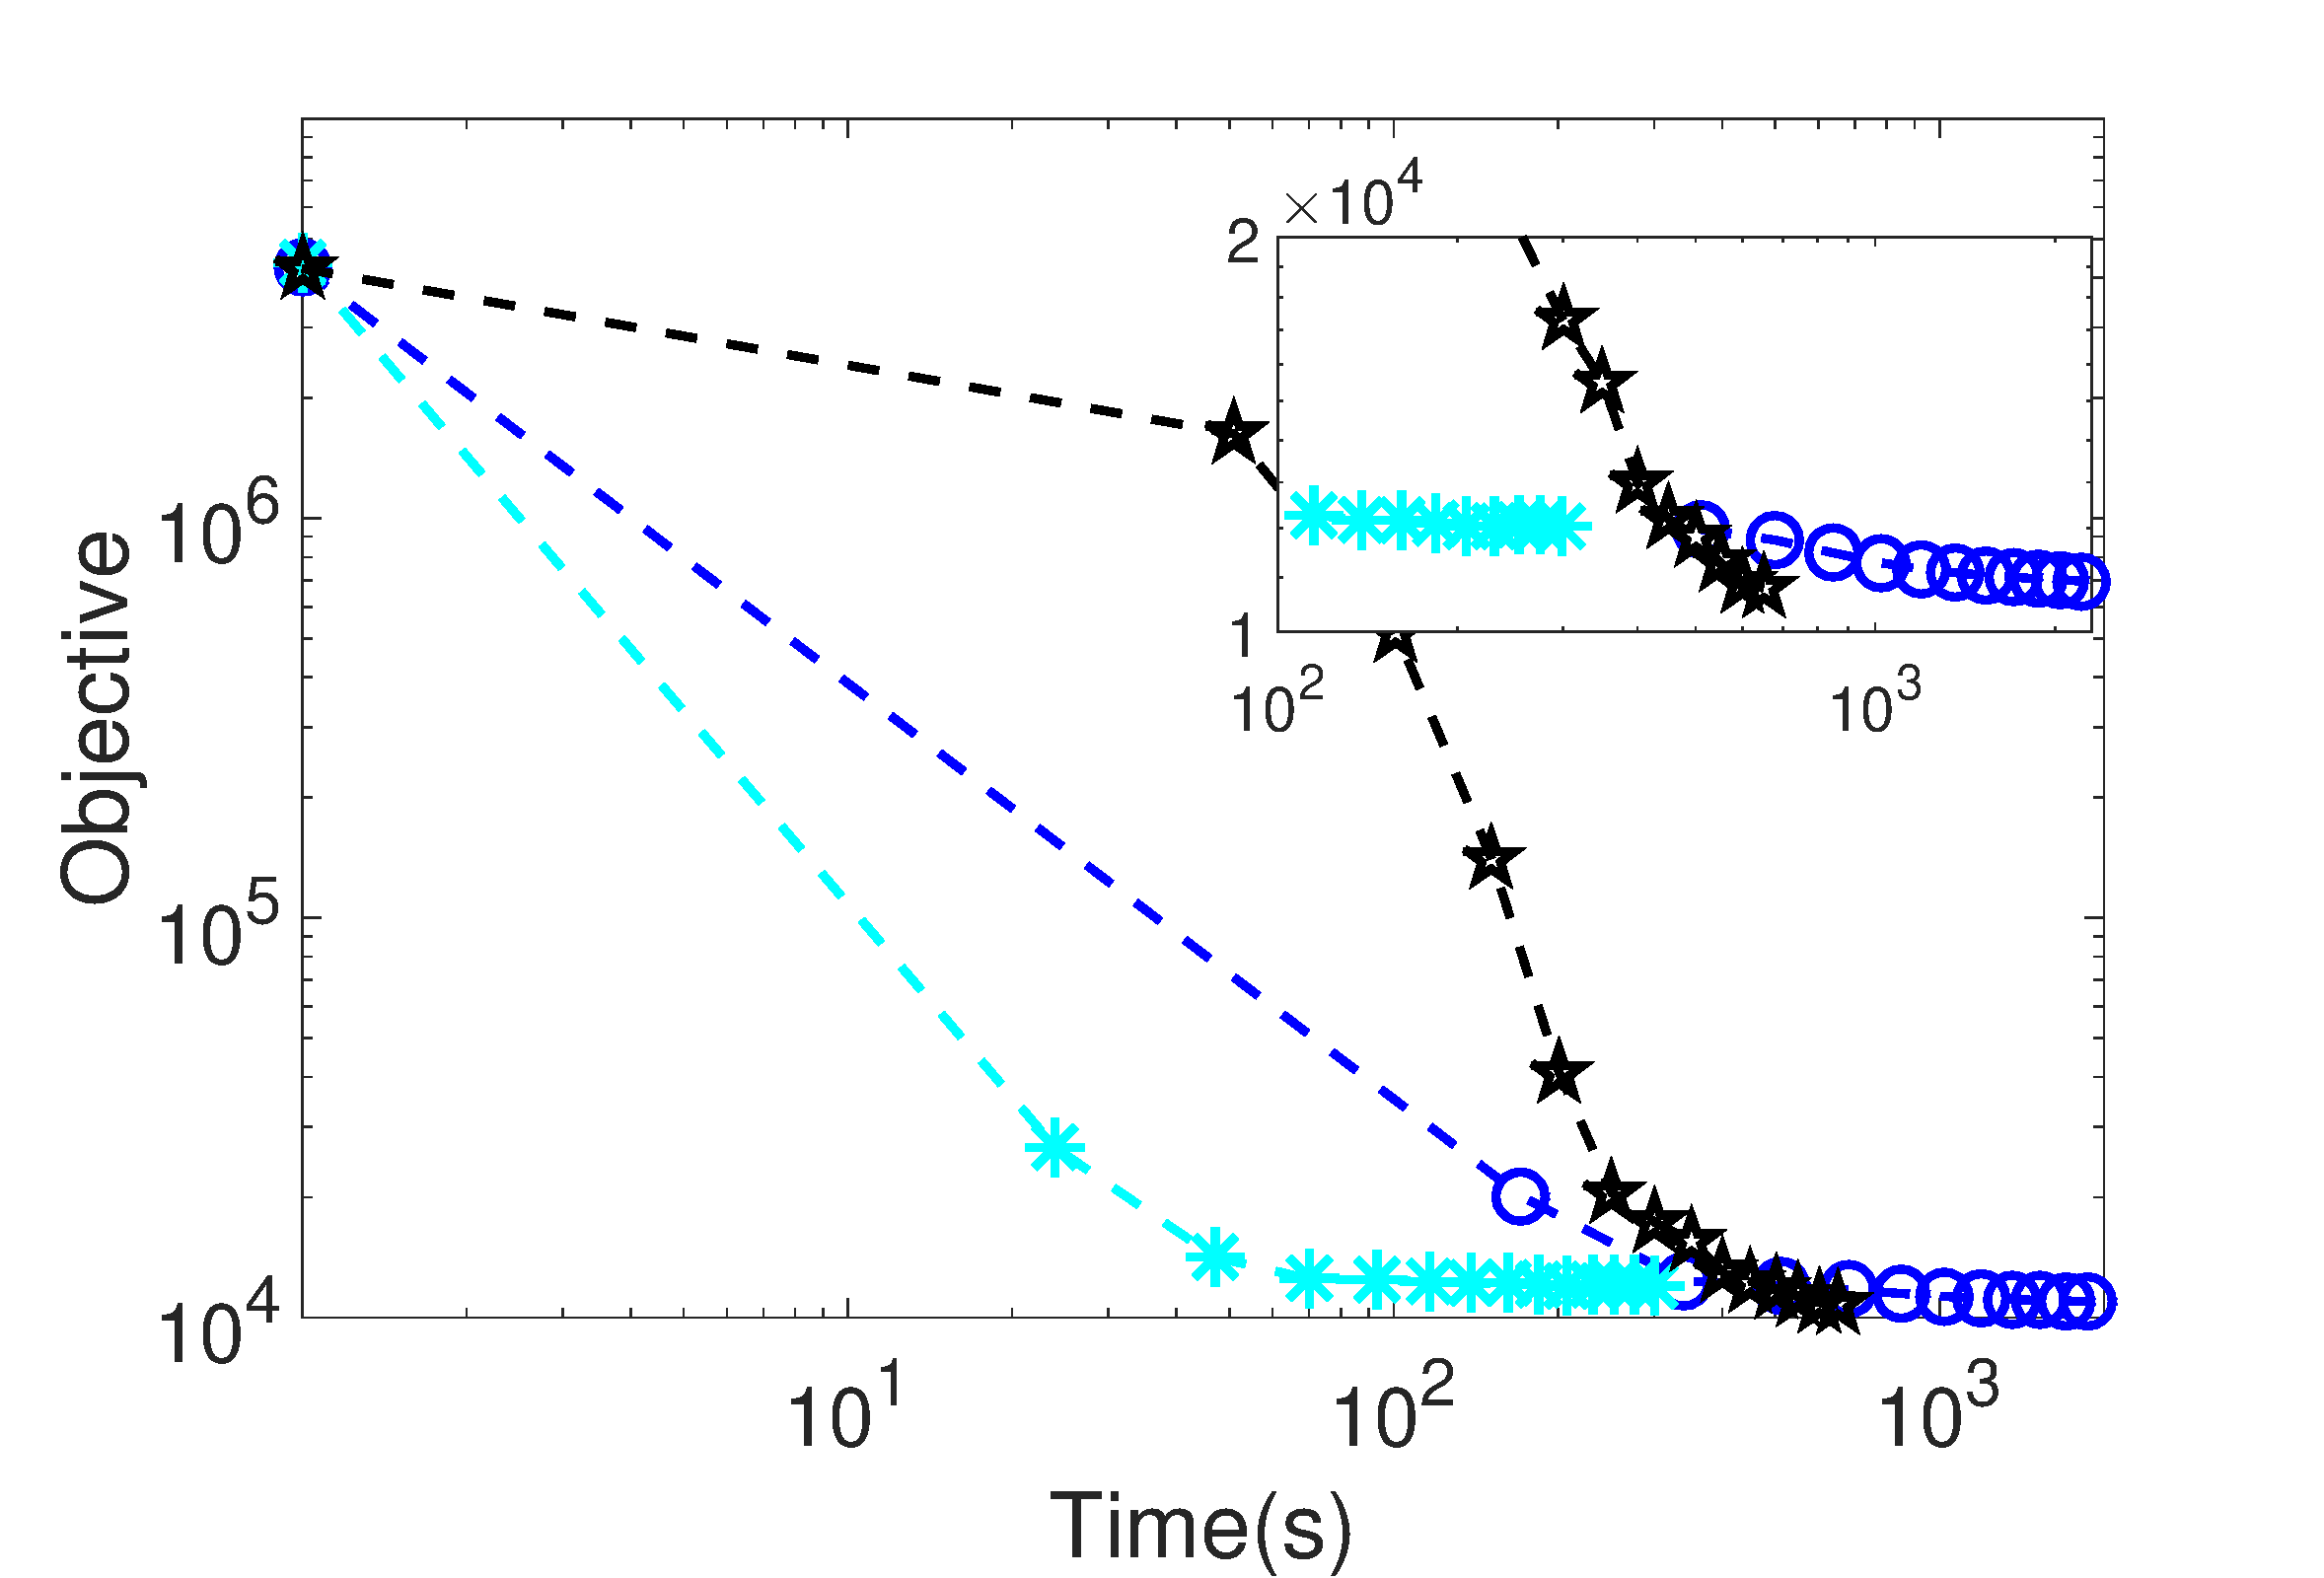
\includegraphics[width=1\linewidth]{figure/timeVSobj-city.pdf}
\end{subfigure}

\centering
\begin{subfigure}{0.49\textwidth}
  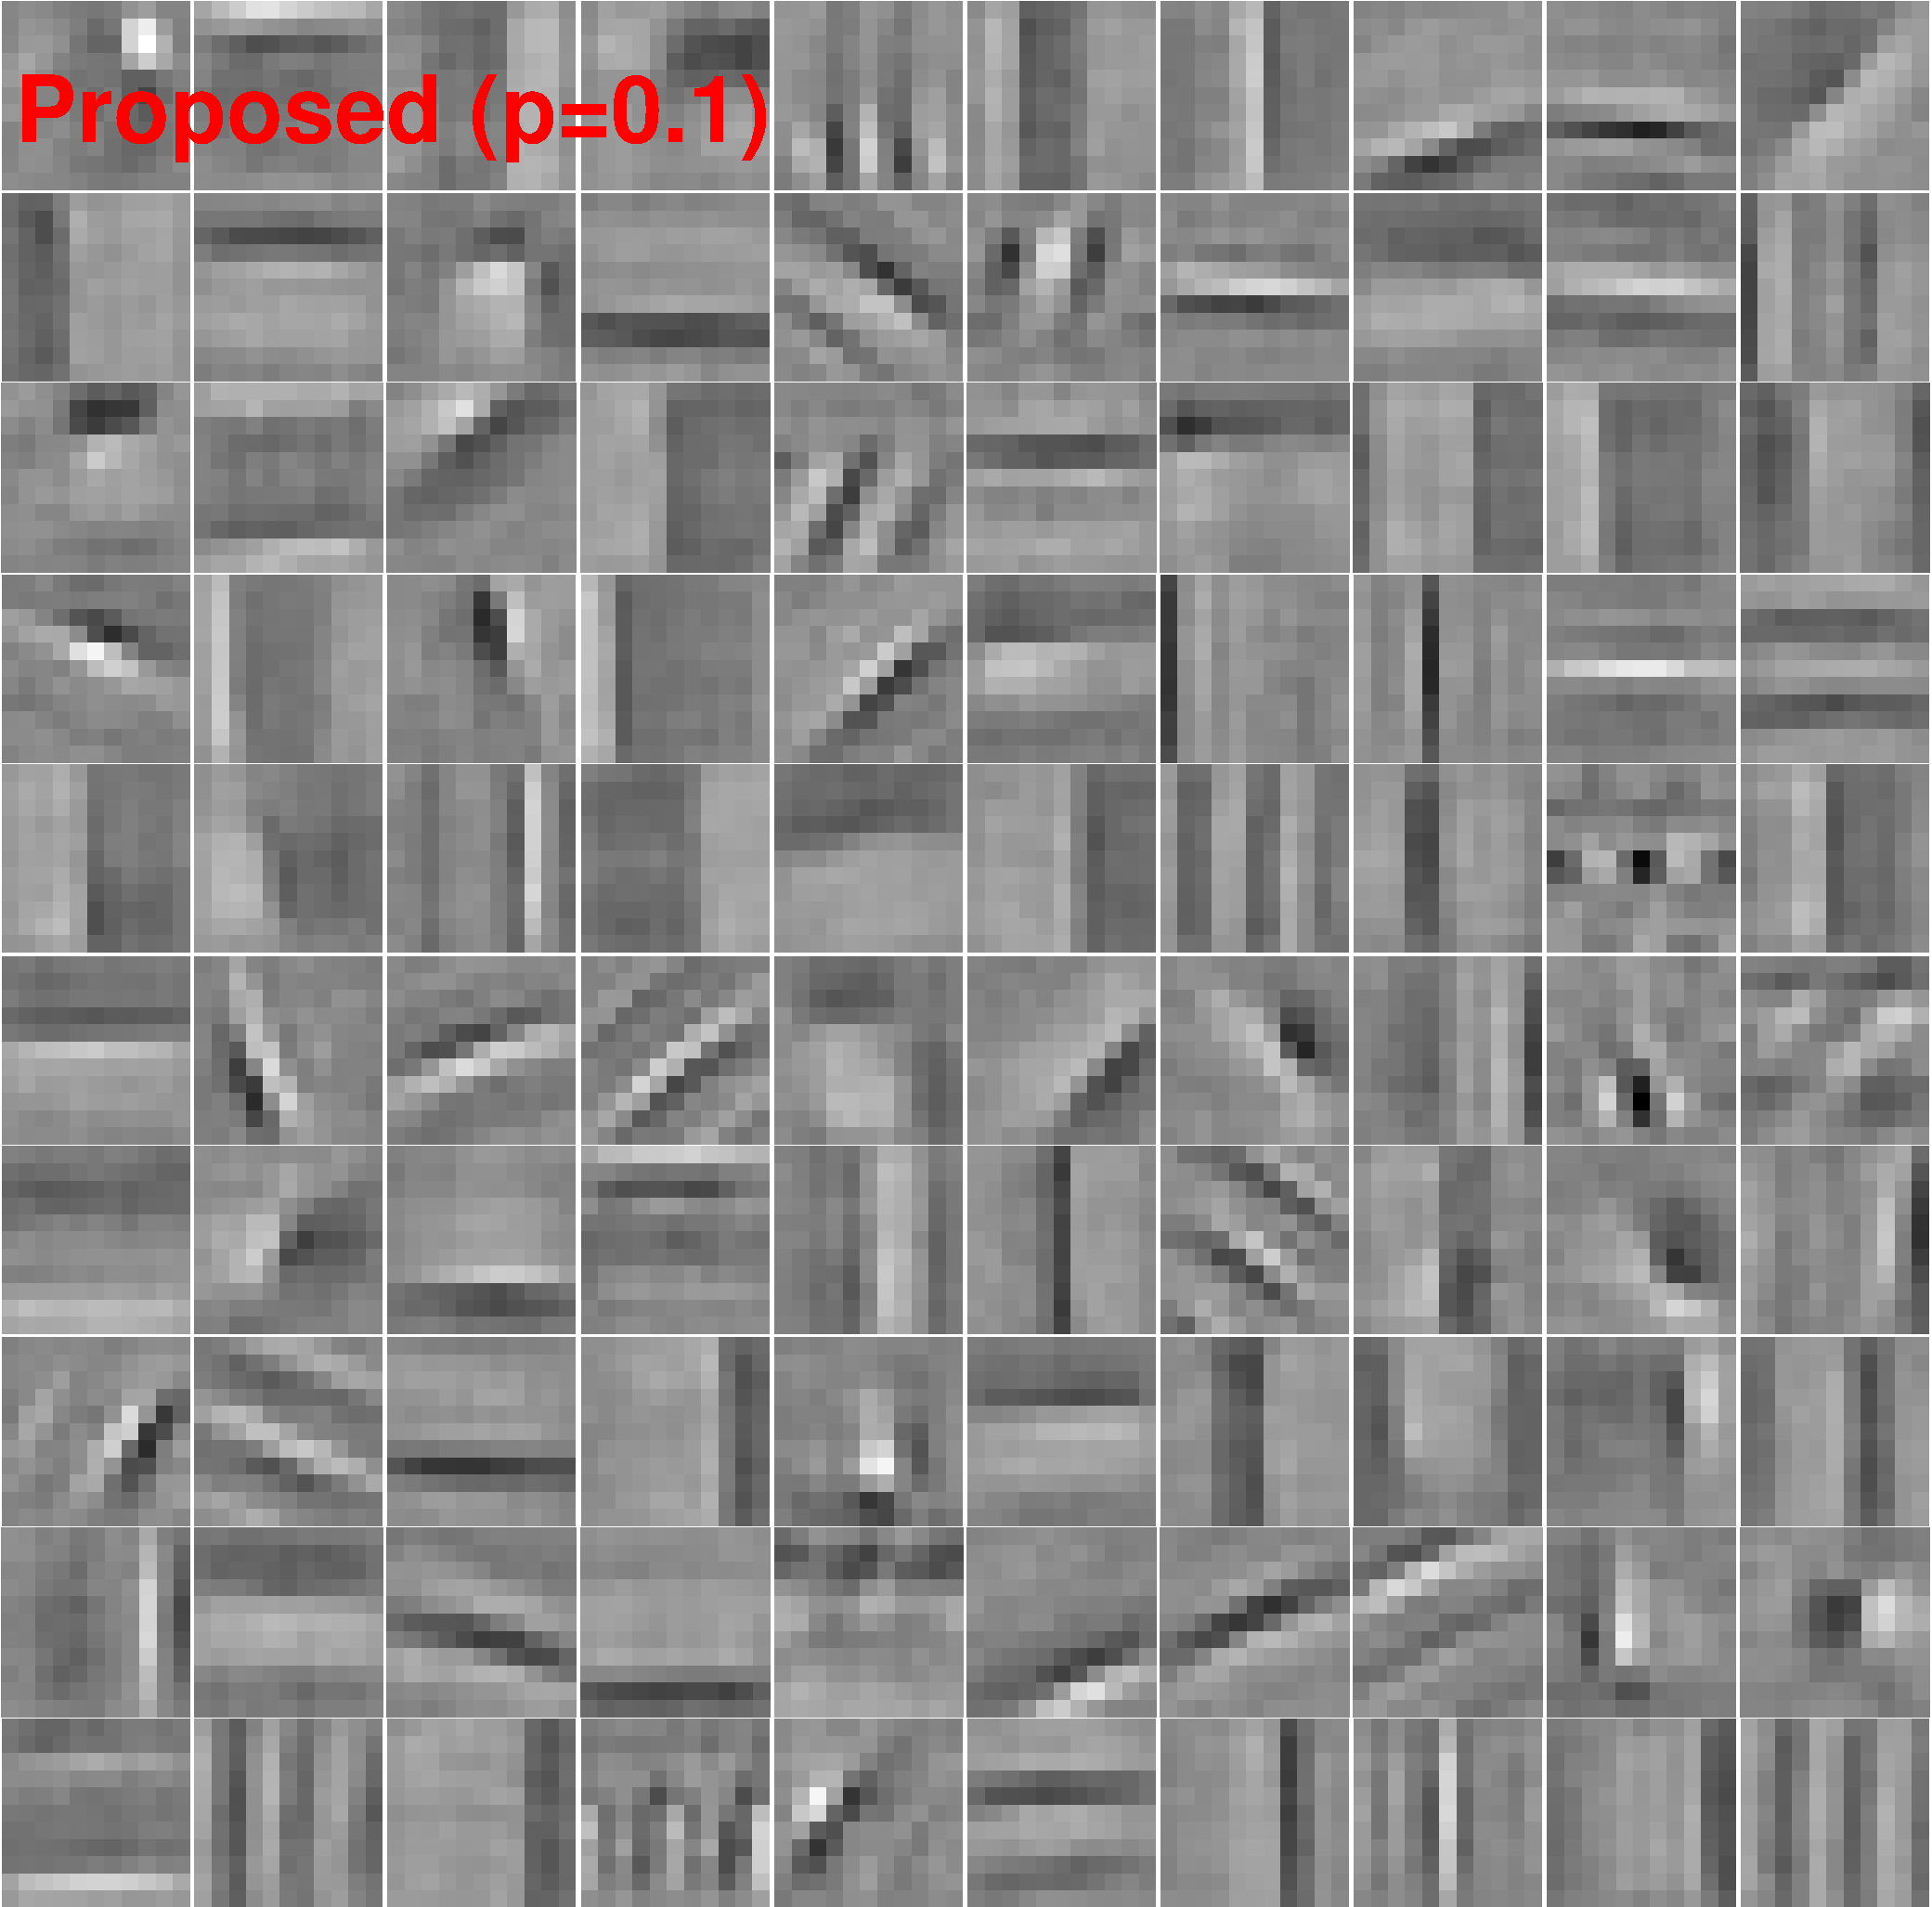
\includegraphics[width=1\linewidth]{figure/batchCity100.pdf}
\end{subfigure}
\begin{subfigure}{0.49\textwidth}
  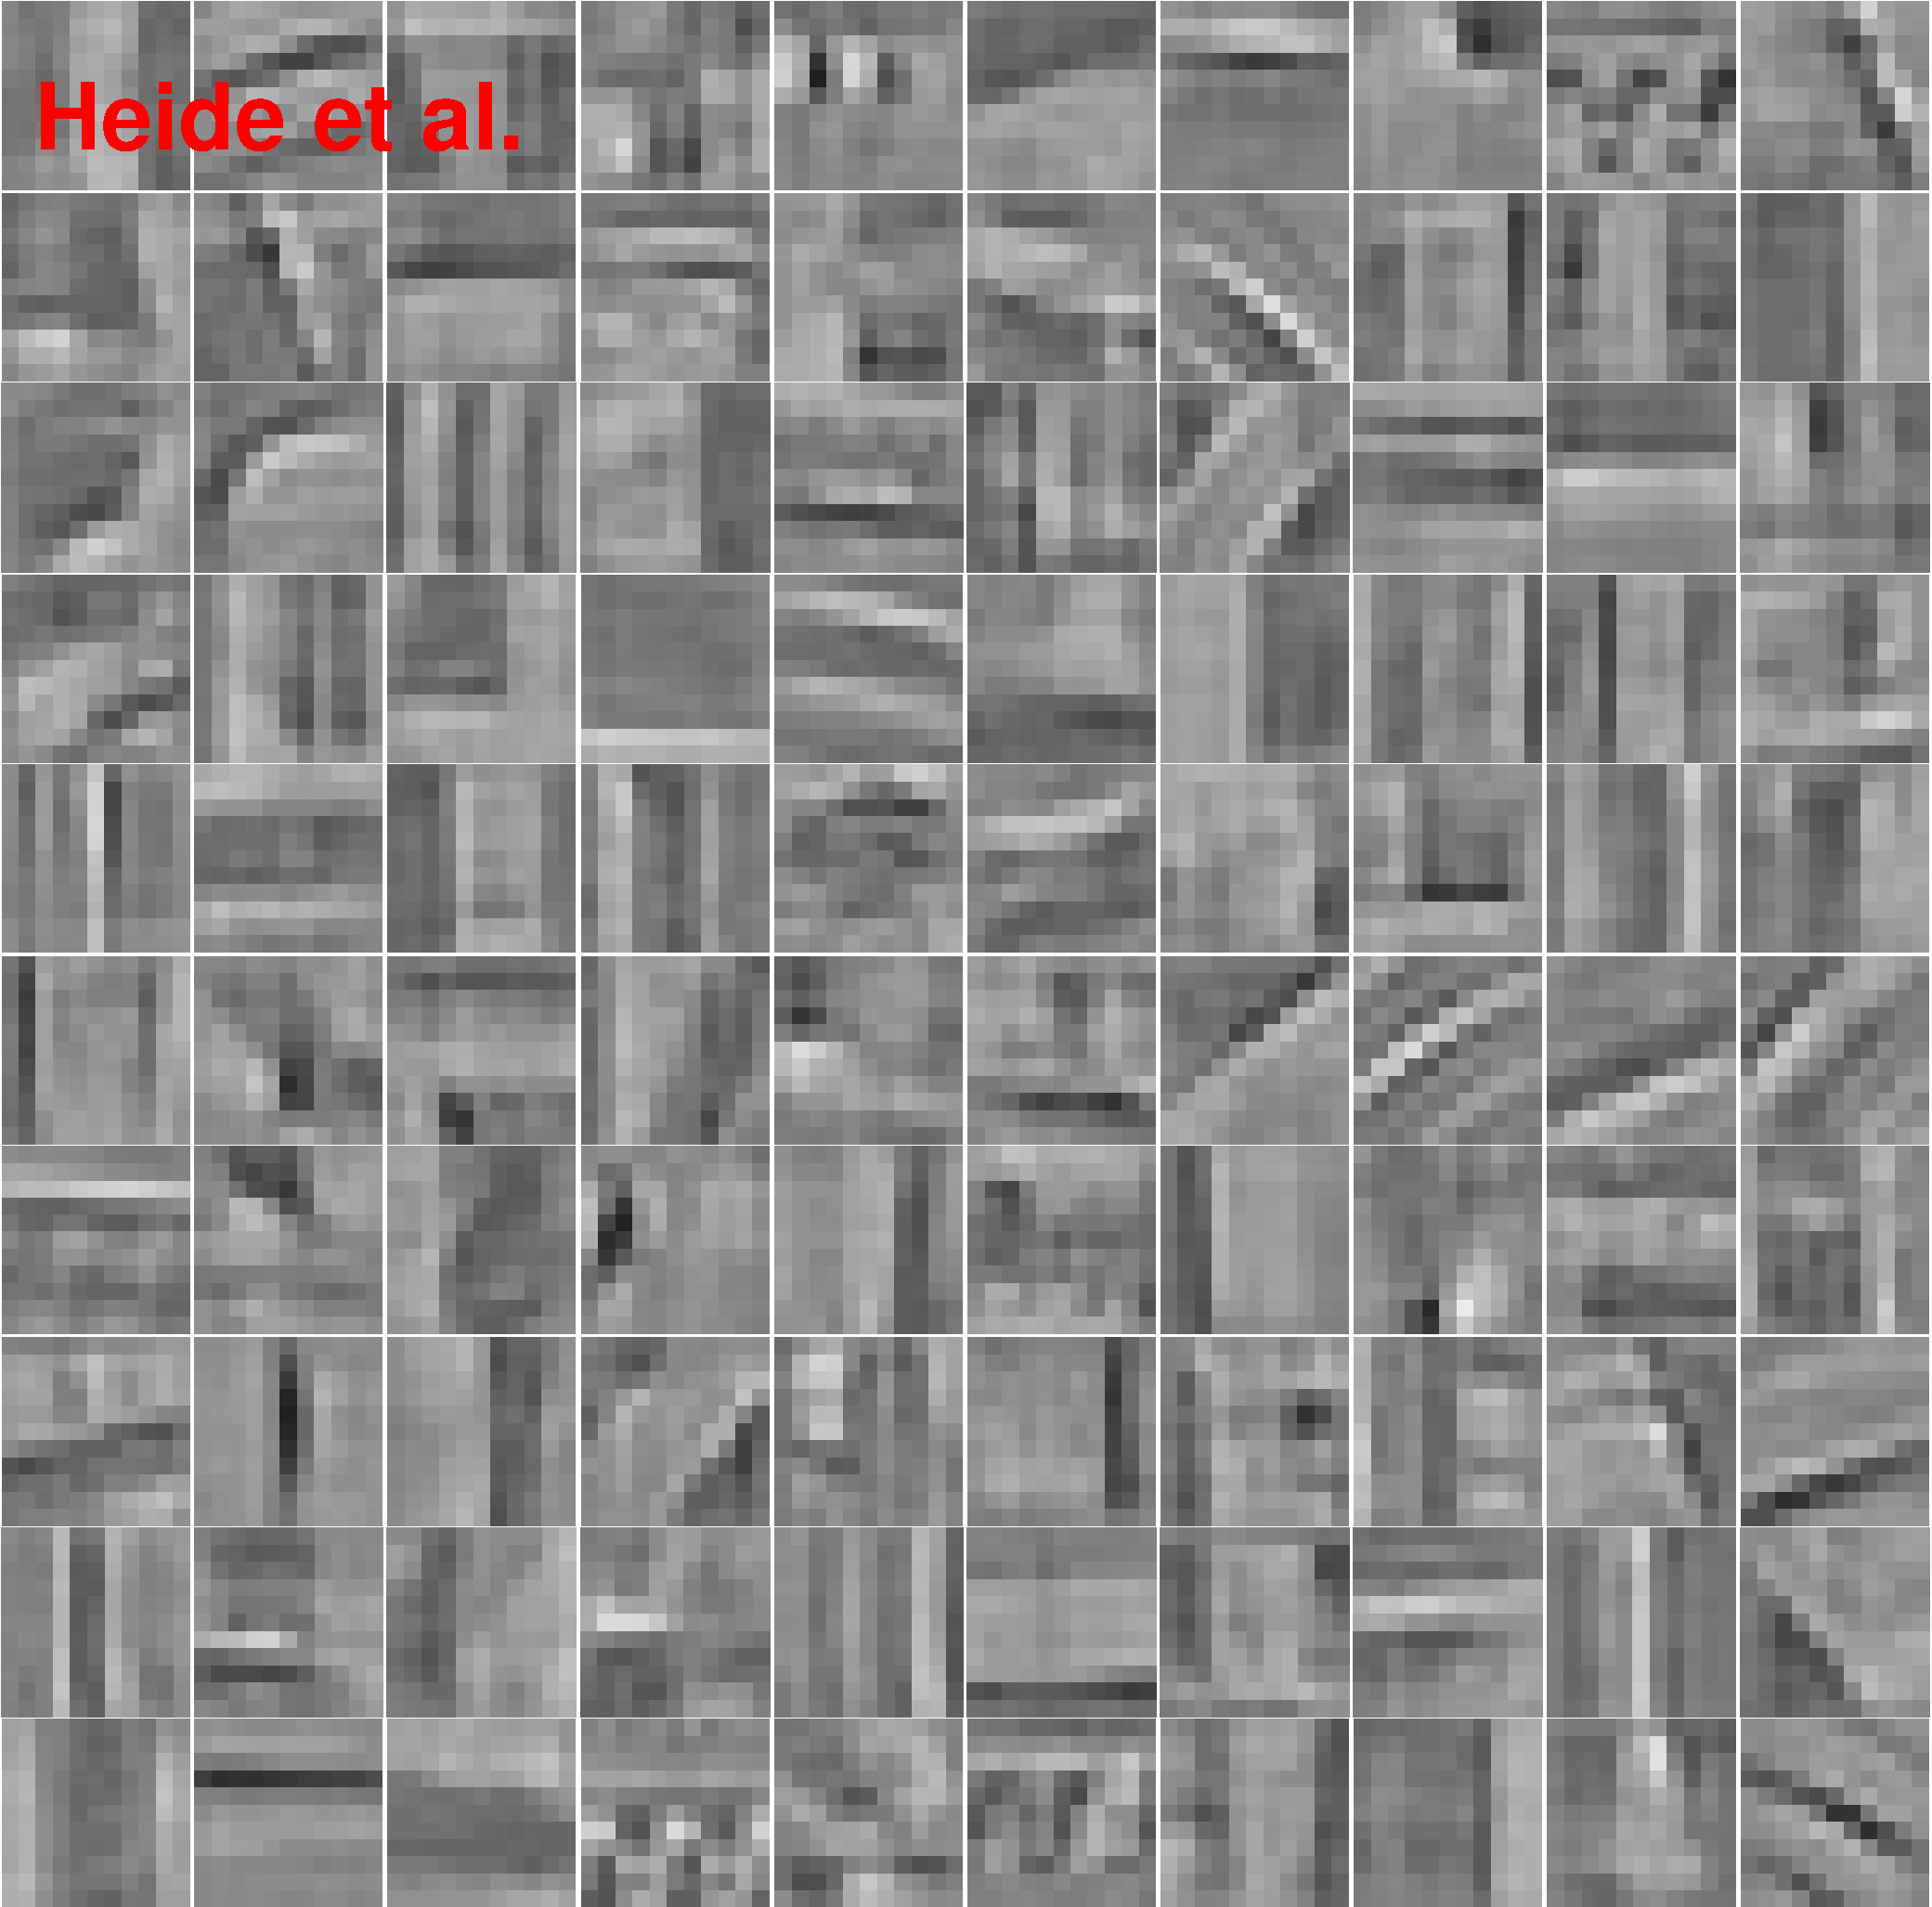
\includegraphics[width=1\linewidth]{figure/heideCity100.pdf}
\end{subfigure}
\vspace{0.2cm}

    \resizebox{0.8\linewidth}{!}{
        \begin{tabular}{|c||c|c|c|c|c|c|c|c|c|c|}
            \cline{1-11}
            Image & 1 & 2 & 3 & 4 & 5 & 6 & 7 & 8 & 9 & 10 \\
            \hline
            PSNR~[10] & 29.67 & \textbf{28.14} & 29.58 & 29.69 & 28.74 & 29.43 & 27.89  & 30.13 & 27.03 & 30.61 \\
            \hline
            PSNR ours & \textbf{29.78} & \textbf{28.14} & \textbf{29.67}  & \textbf{29.85} & \textbf{28.88} & \textbf{29.95} & \textbf{27.97} & \textbf{30.37} & \textbf{27.14} & \textbf{30.89} \\
            \hline
        \end{tabular} }

\caption{Experimental results obtained on the city dataset. Top: Convergence comparison between the-state-of-art batch method and SBCSC with different subsampling probability. Middle: Learned filters by SBCSC with $p=0.1$ and the comparable method. Even though these dictionaries look similar, our method learns more smooth filters. Compared to the learned filters in Fig.~1 of the main manuscript, they have different representations of the dictionaries, where data-specific features are learned from handful training images. Bottom: Numerical comparisons of the reconstruction quality obtained by the presented filters in the image inpainting application.}
\label{fig:subsampleResult-city}
\end{figure*}

We then compare SOCSC with the state-of-the-art online algorithm on city dataset, the results of which are shown in Fig.\ \ref{fig:onlineSmall-city}. Similar to the results presented in Fig.~3 of the main manuscript, our method obtains comparable outcomes, meanwhile, achieves roughly $6 \times$ speedup.

\section{Over-complete Dictionary and Large Datasets}
\begin{figure*}[h]
\centering
\begin{subfigure}{0.49\textwidth}
  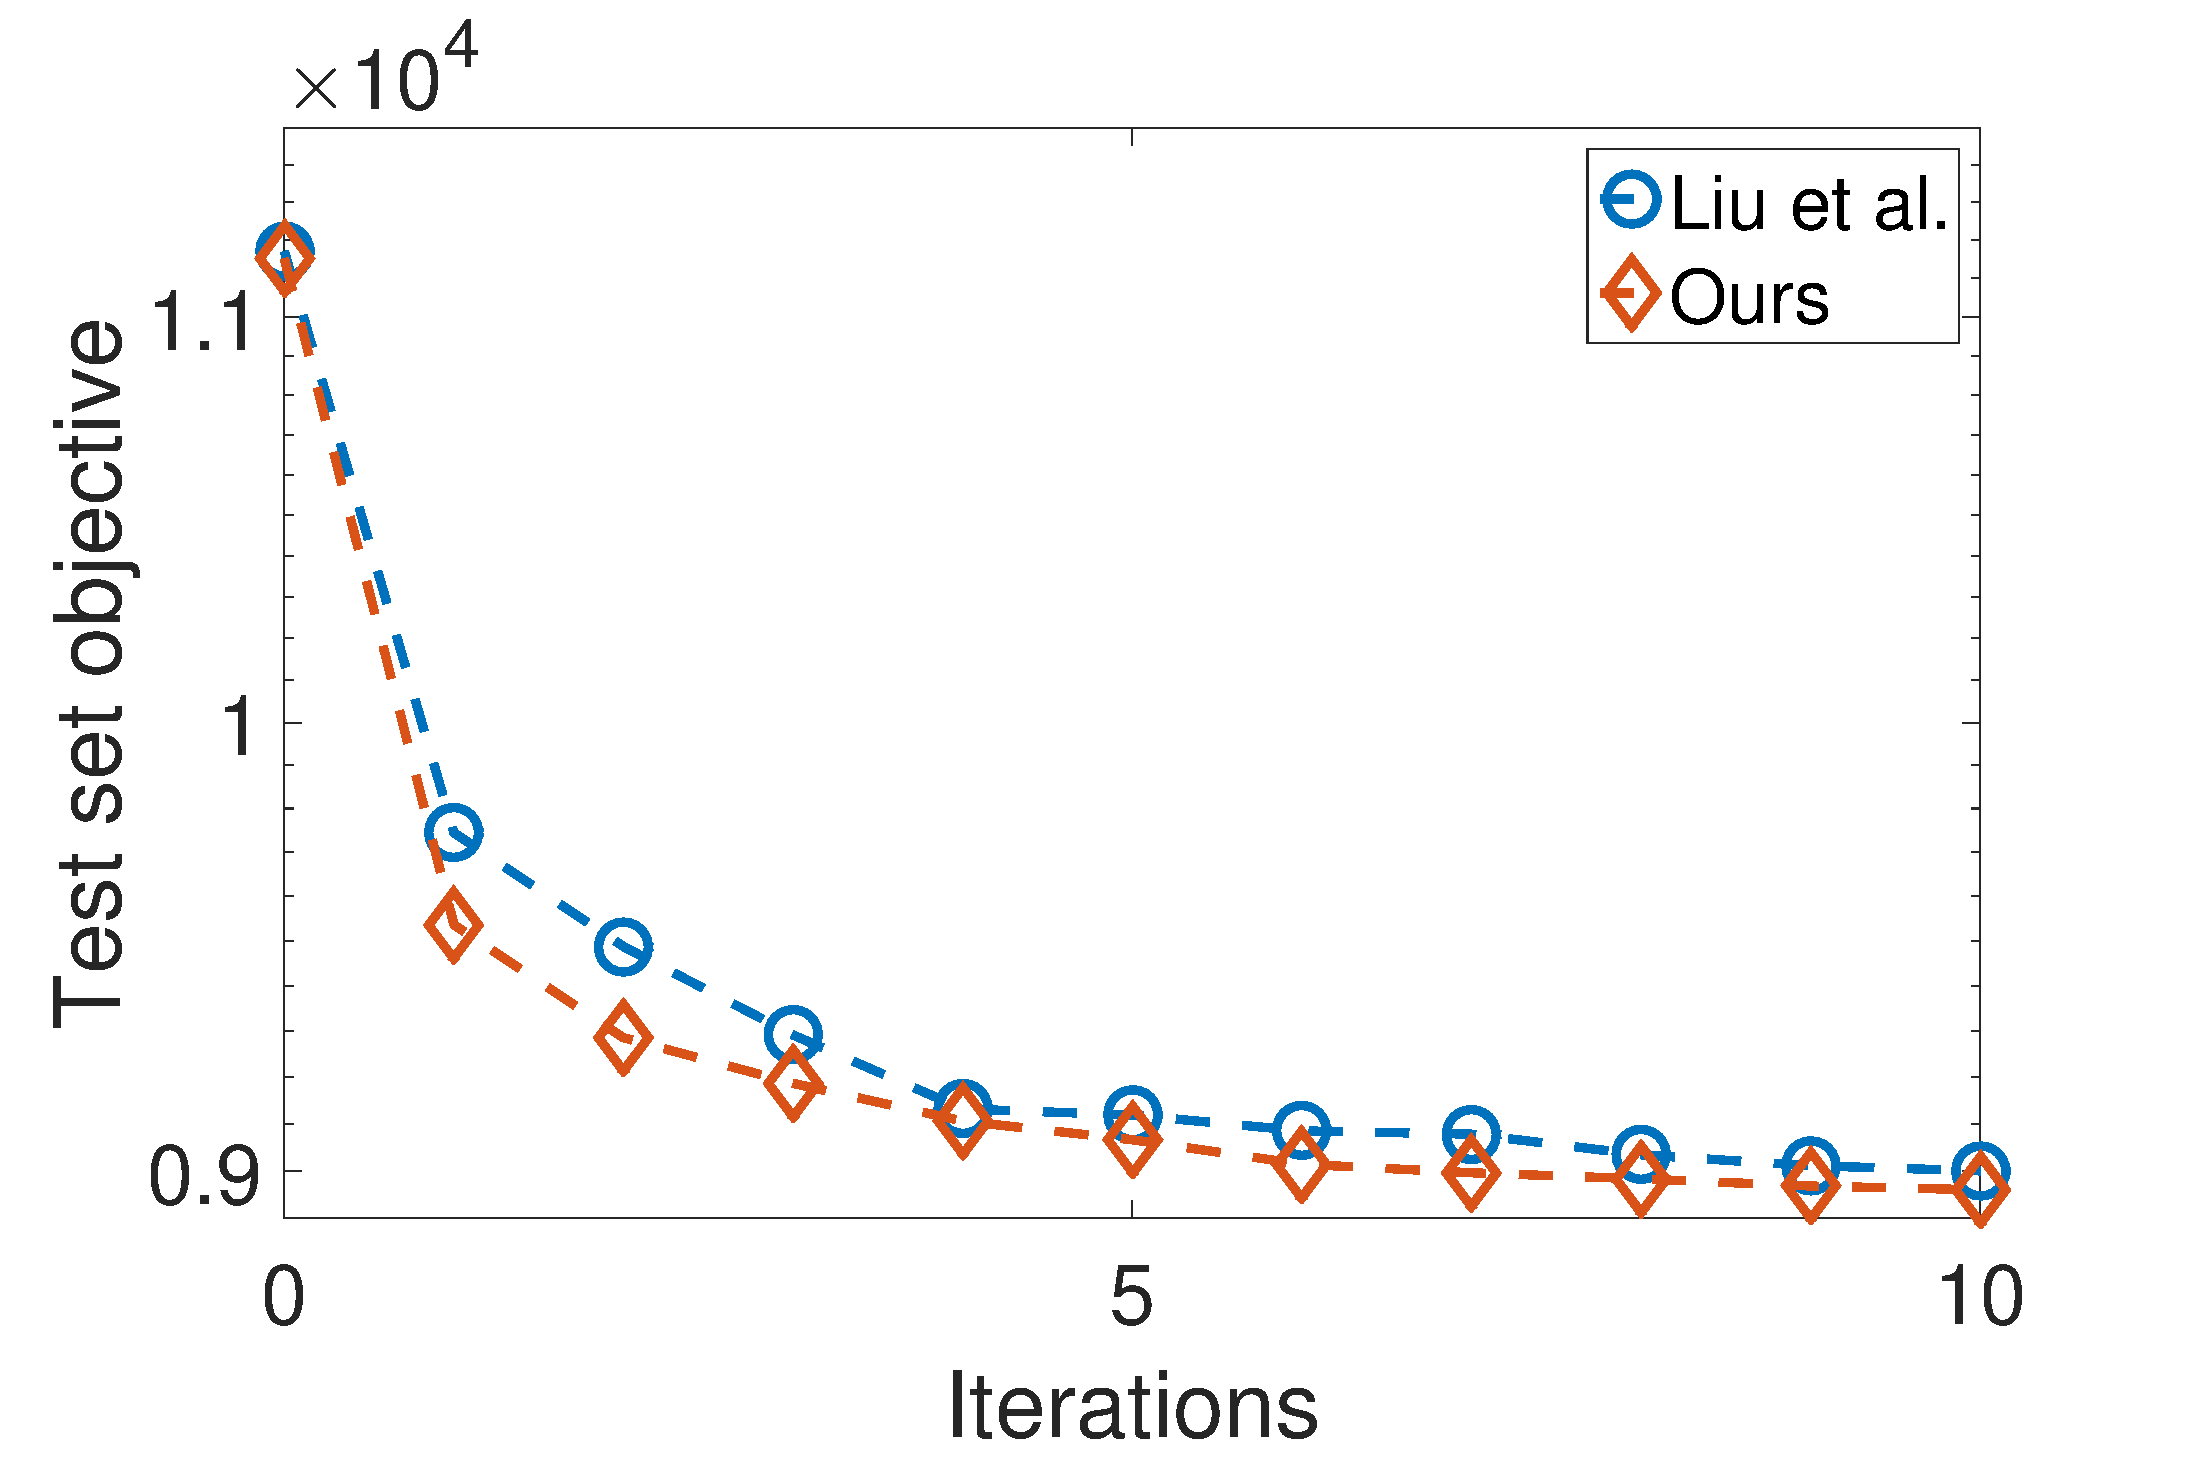
\includegraphics[width=1\linewidth]{figure/onlineVSliu-ite.pdf}
\end{subfigure}
\begin{subfigure}{0.49\textwidth}
  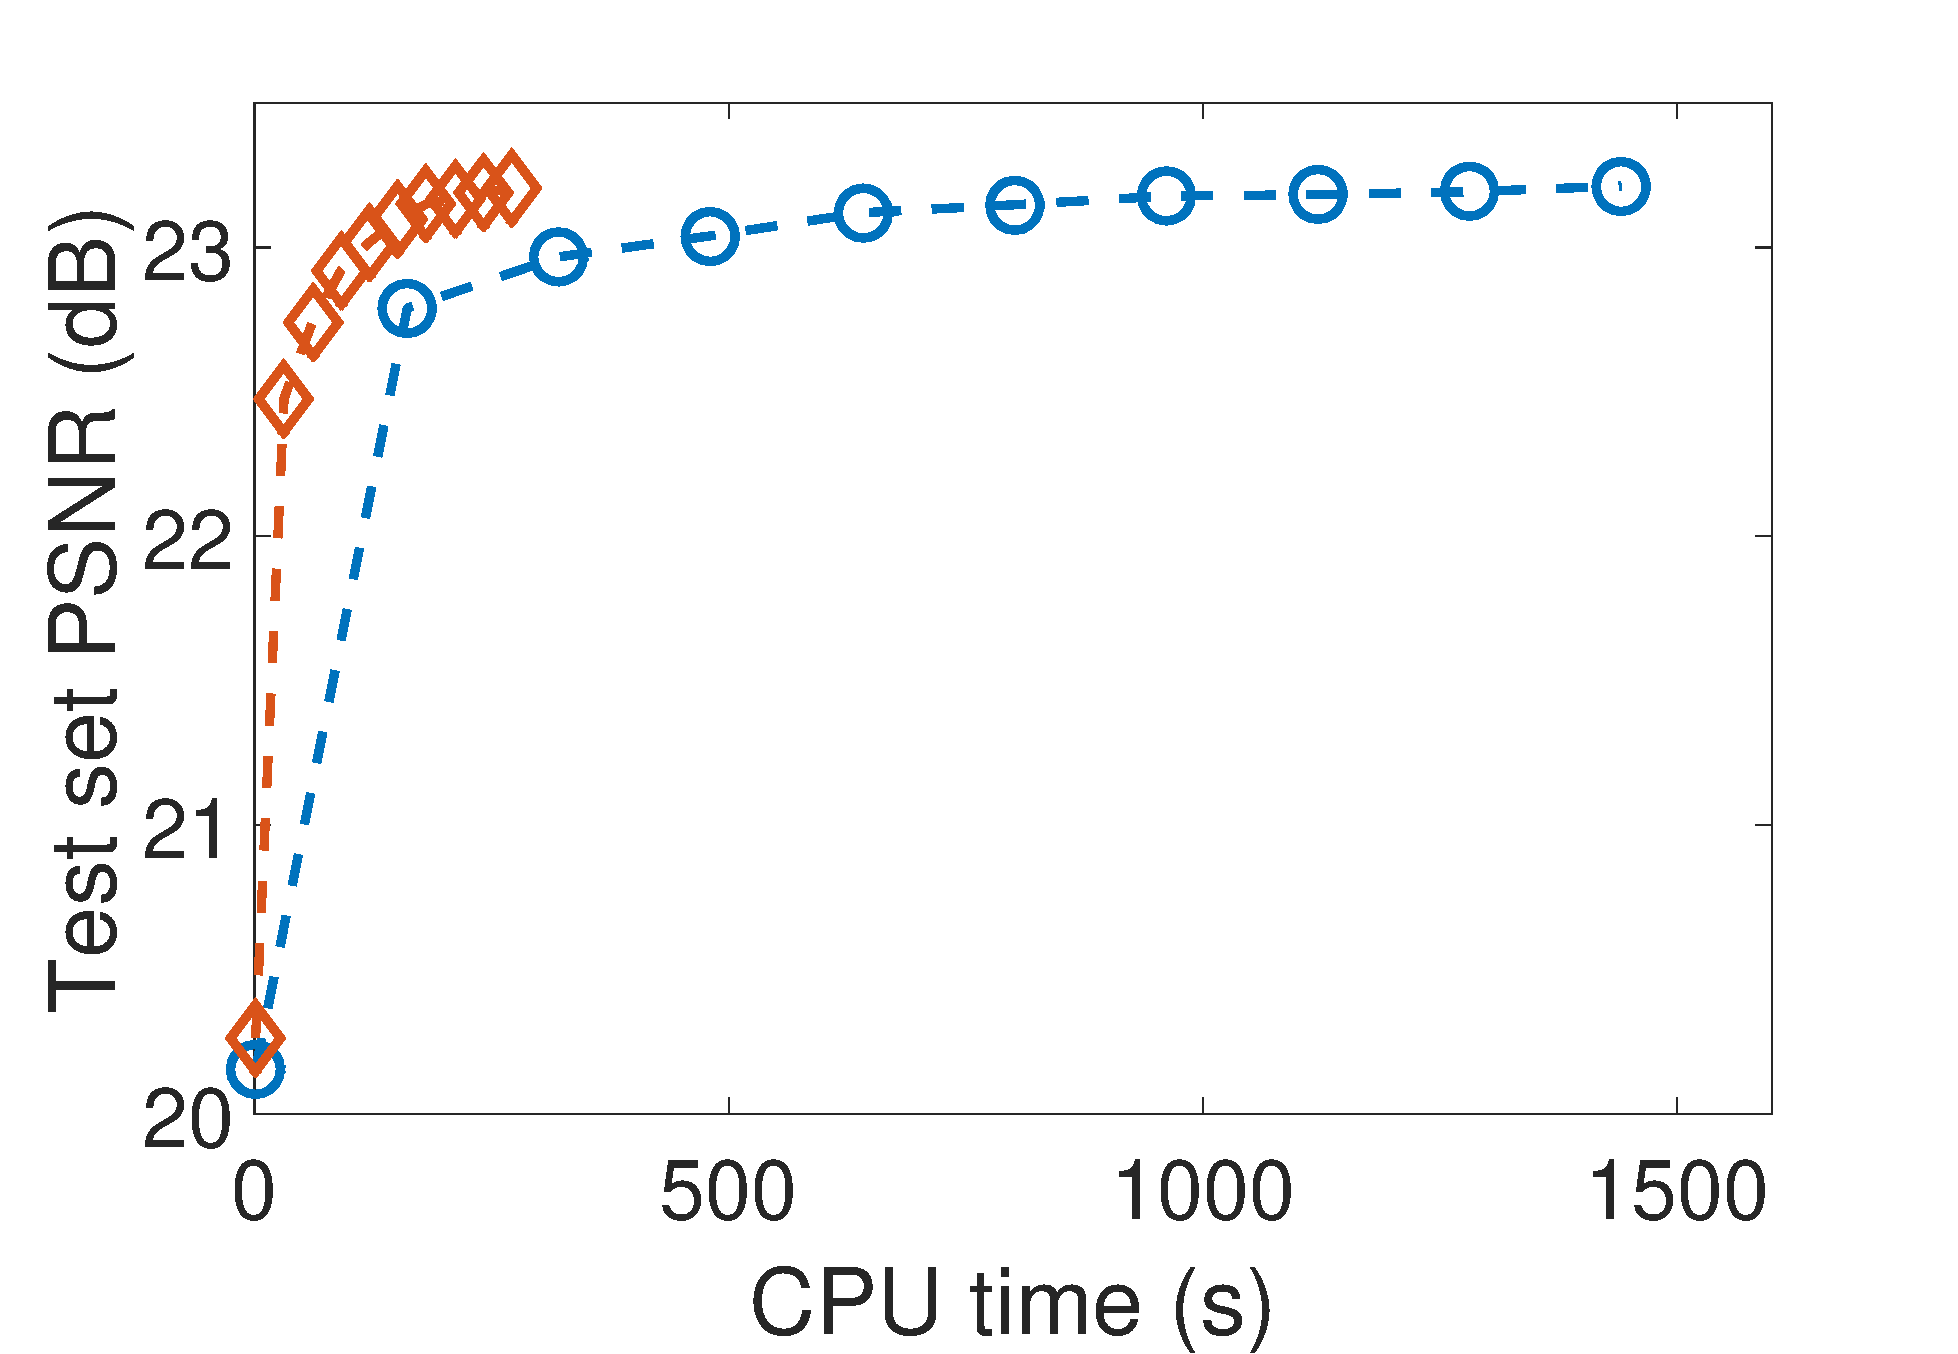
\includegraphics[width=1\linewidth]{figure/onlineVSliu-time.pdf}
\end{subfigure}

\caption{Experimental results obtained on city dataset. Left: Convergence of the test set objectives for our method (SOCSC) and the state-of-the-art online approach. Right: Testing PSNR with respect to execution time.}
\label{fig:onlineSmall-city}
\end{figure*}

\begin{figure*}[h]
\centering
\begin{subfigure}{0.49\textwidth}
  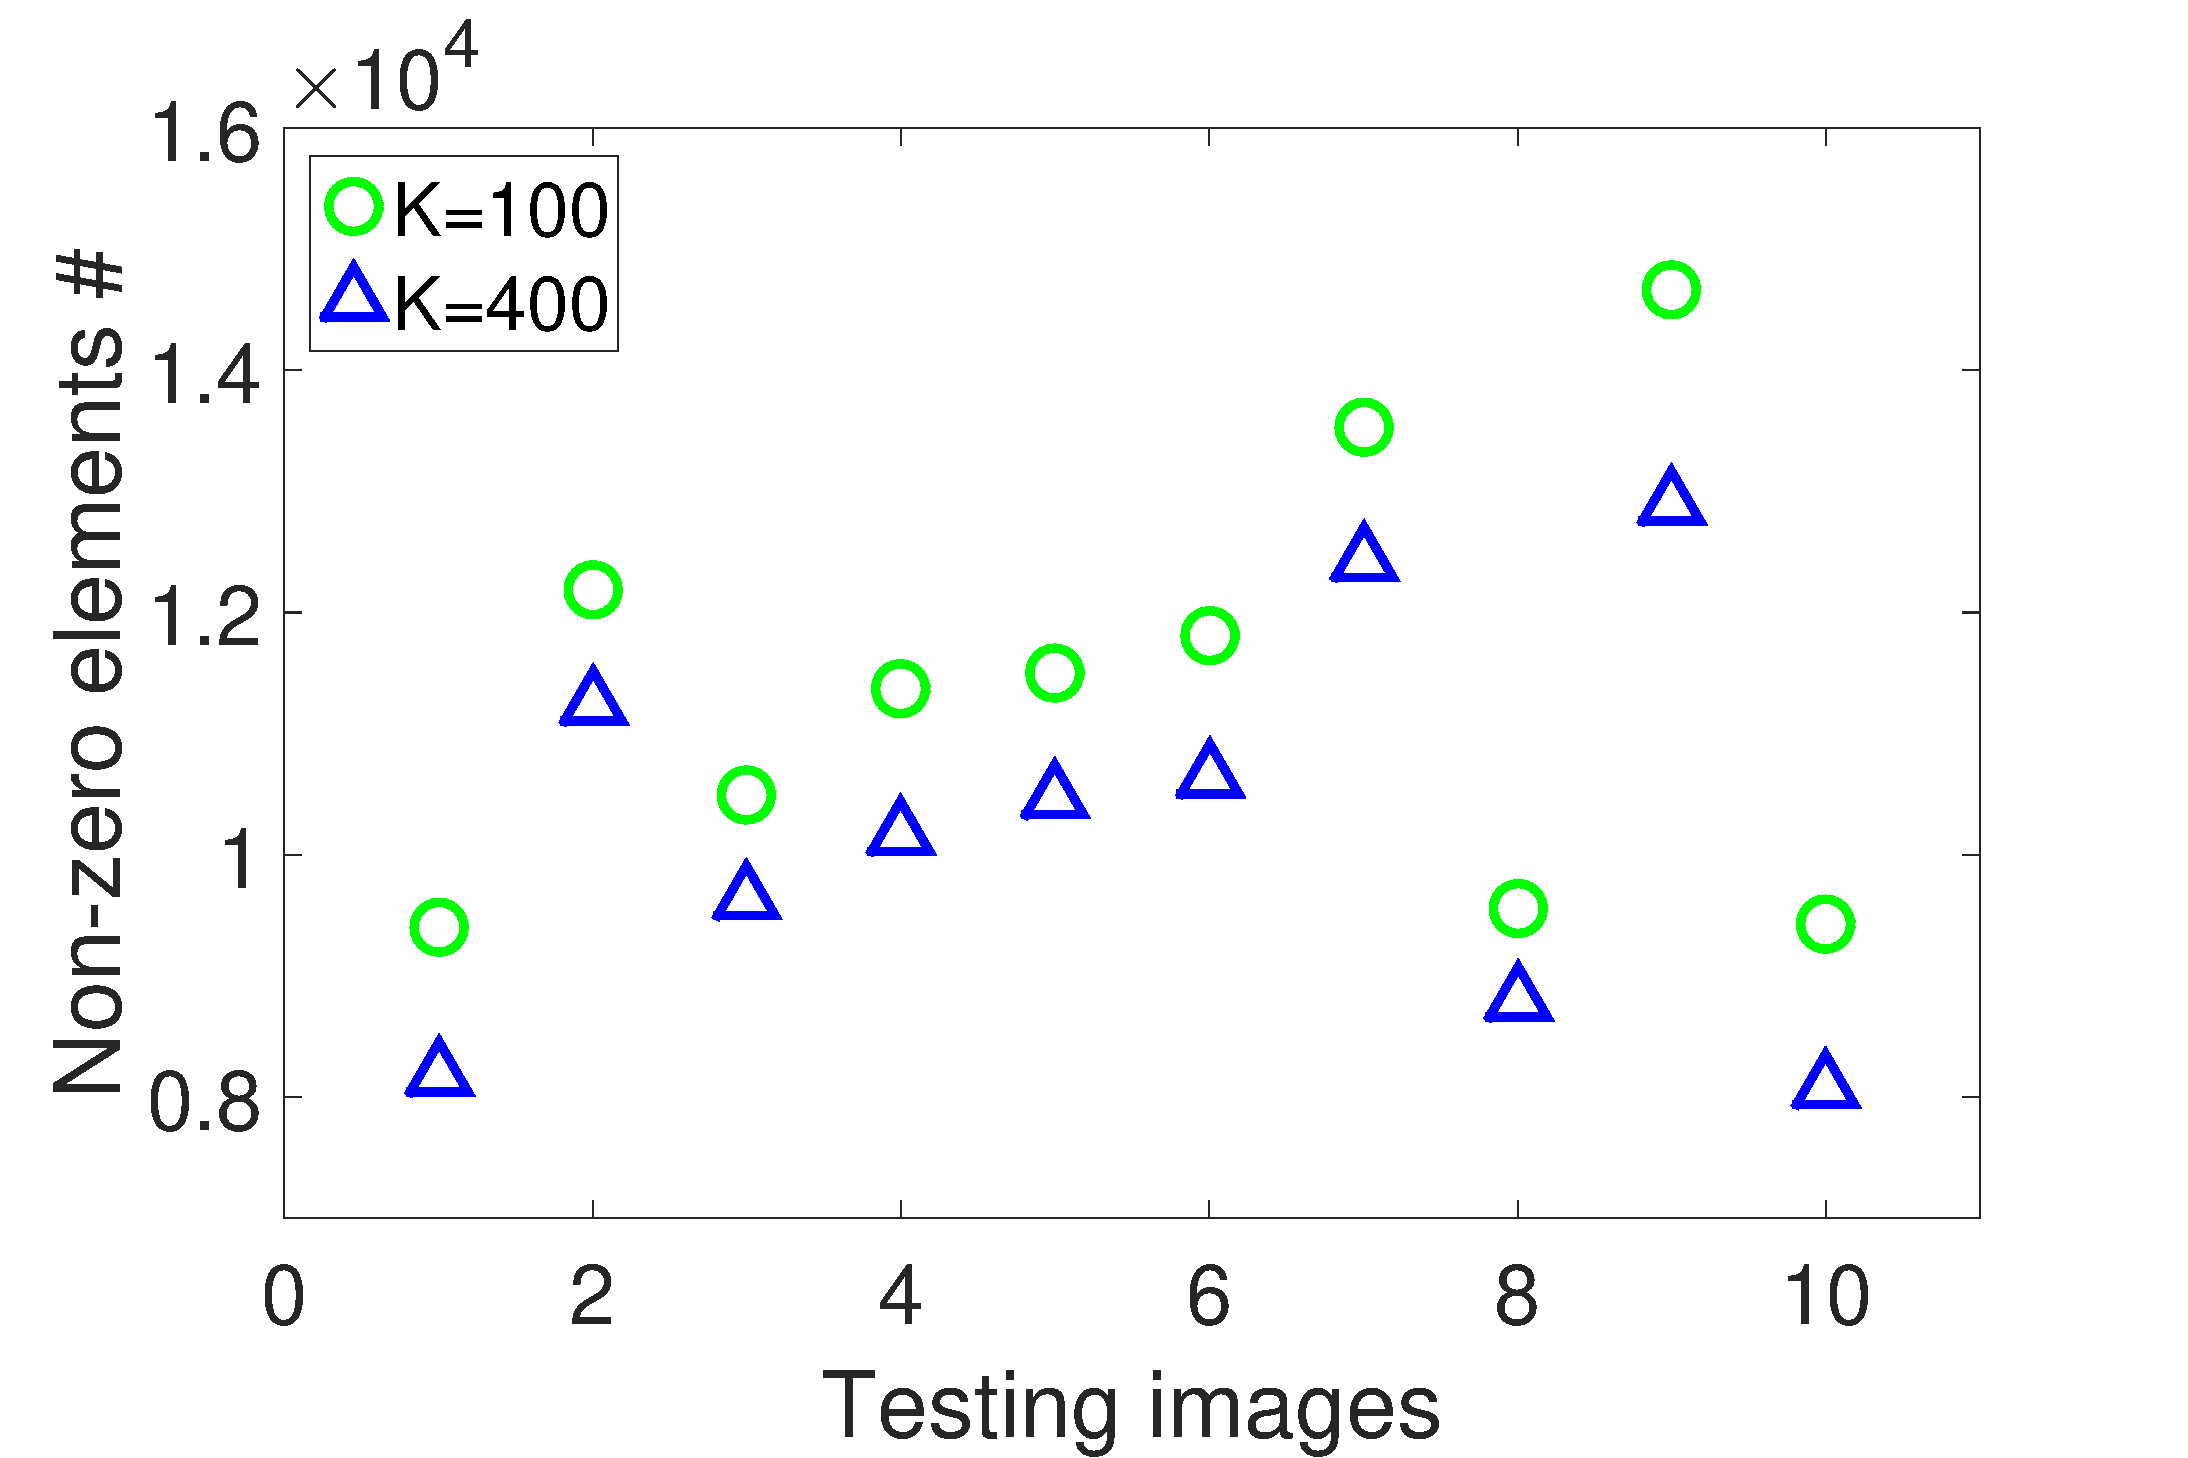
\includegraphics[width=1\linewidth]{figure/nonZeroElement.pdf}
\end{subfigure}
\begin{subfigure}{0.49\textwidth}
  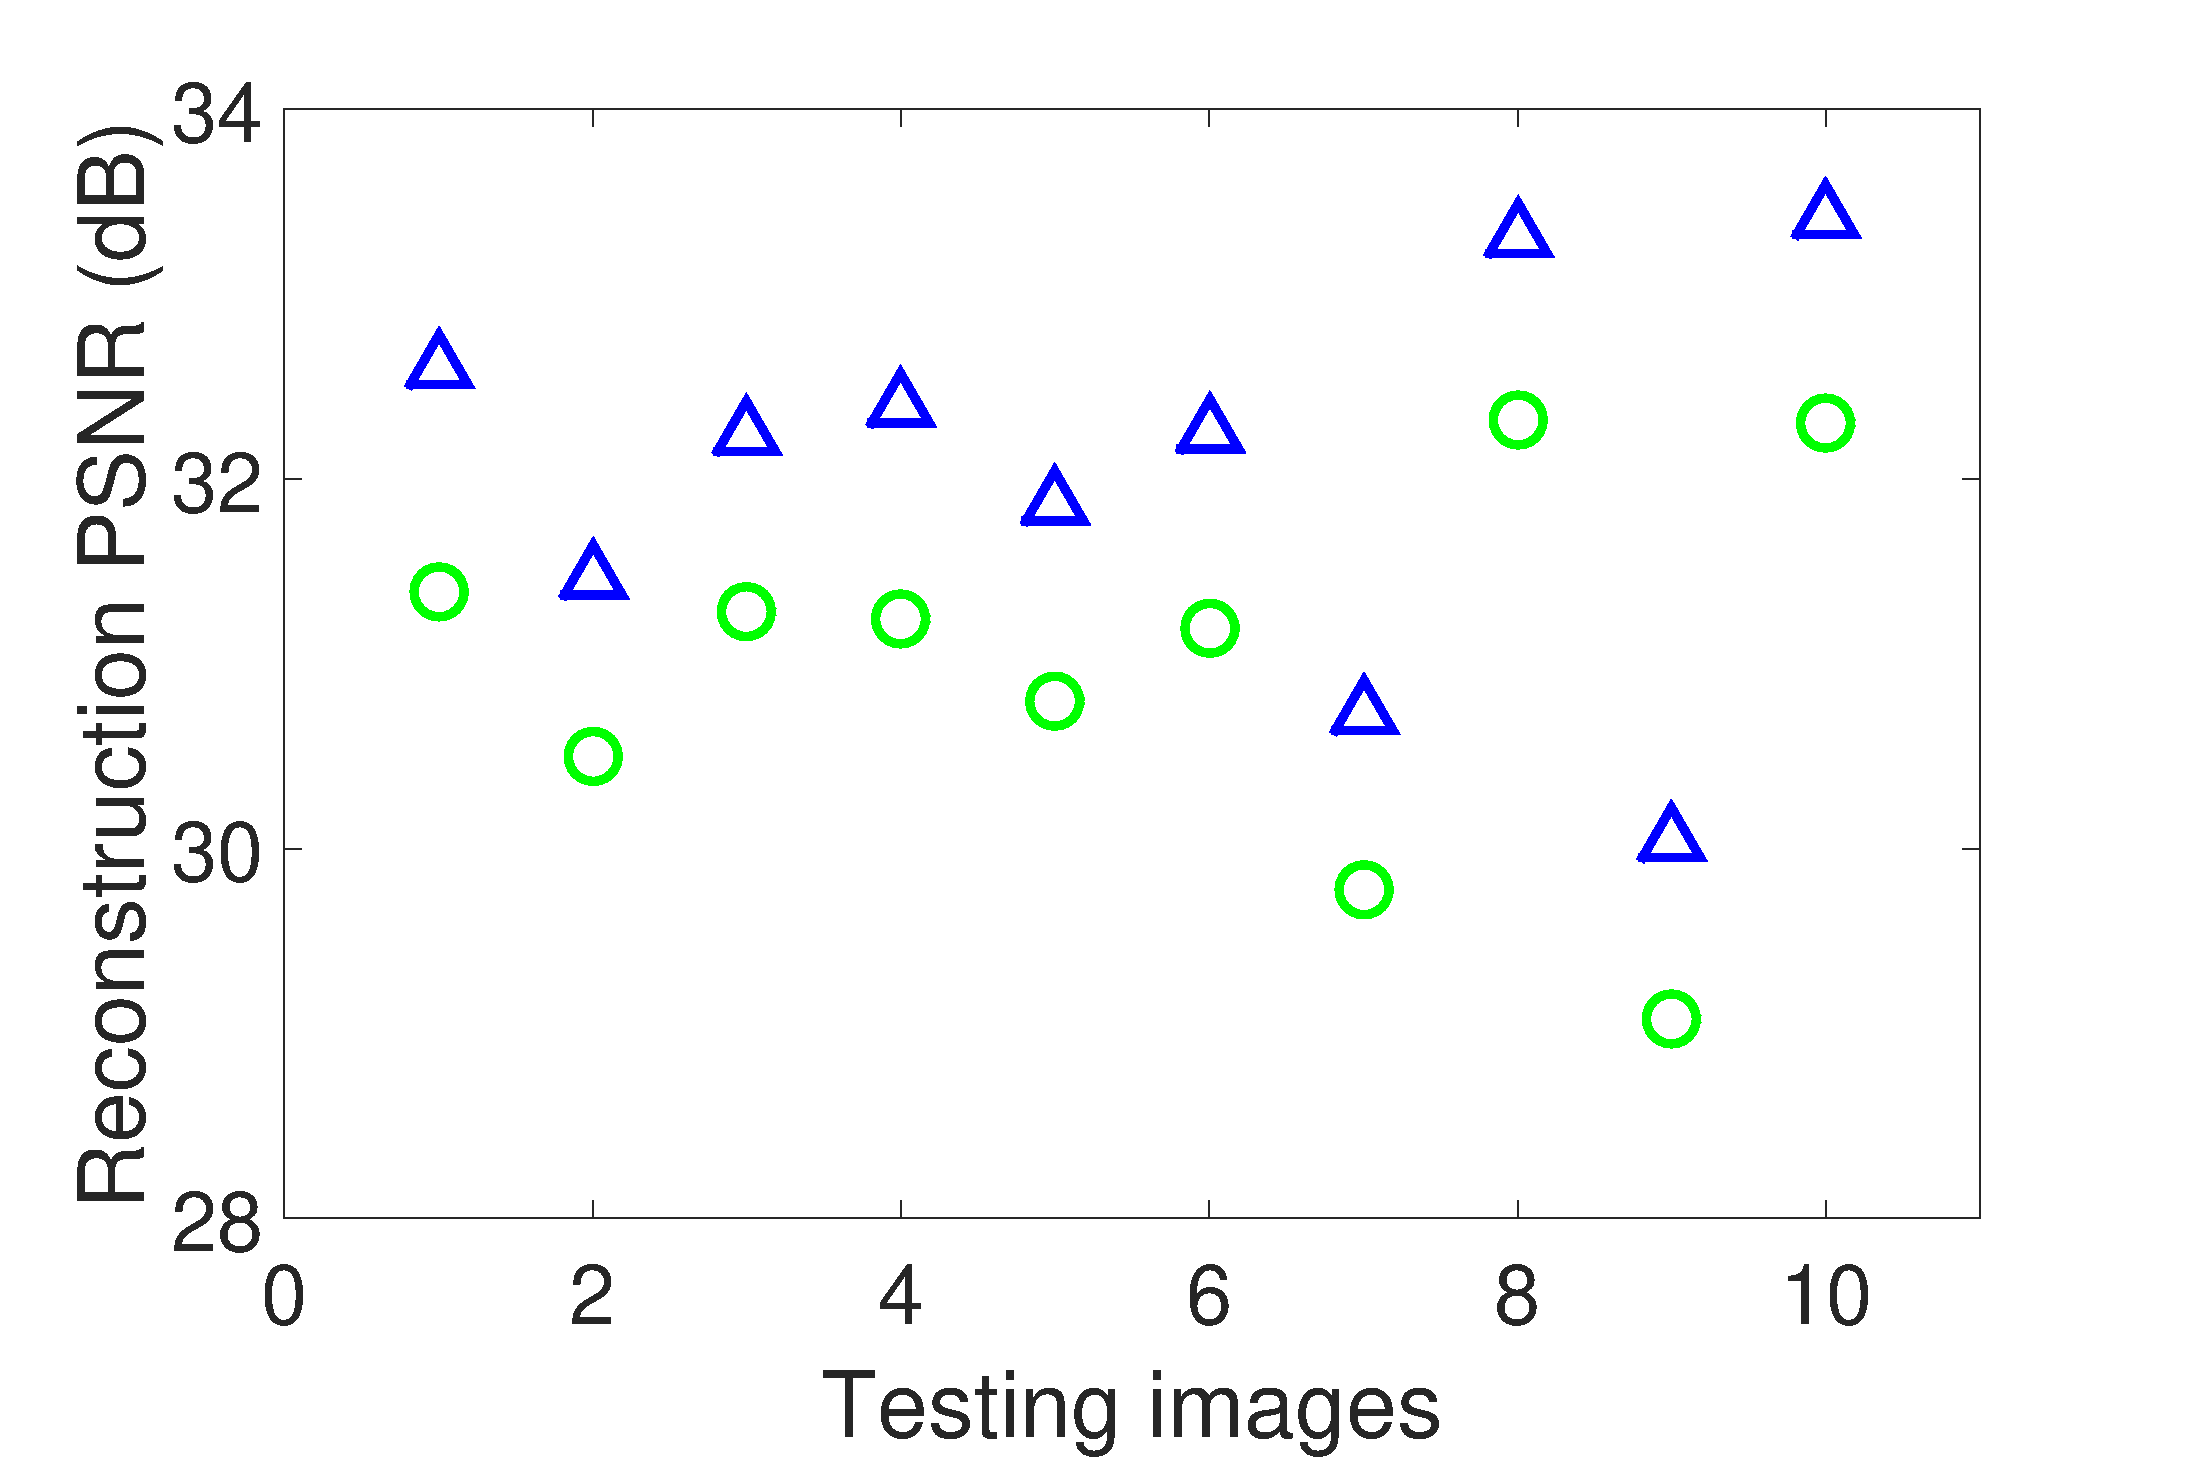
\includegraphics[width=1\linewidth]{figure/reconPSNR.pdf}
\end{subfigure}

\caption{Left: number of non-zero elements in the codes for different images ($10 ~ 256 \times 256$ images). Right: PSNR between the reconstructed images and the original ones.}
\label{fig:overVSunder}
\end{figure*}



\begin{figure*}[h]
\centering
  \begin{subfigure}{0.5\textwidth}
  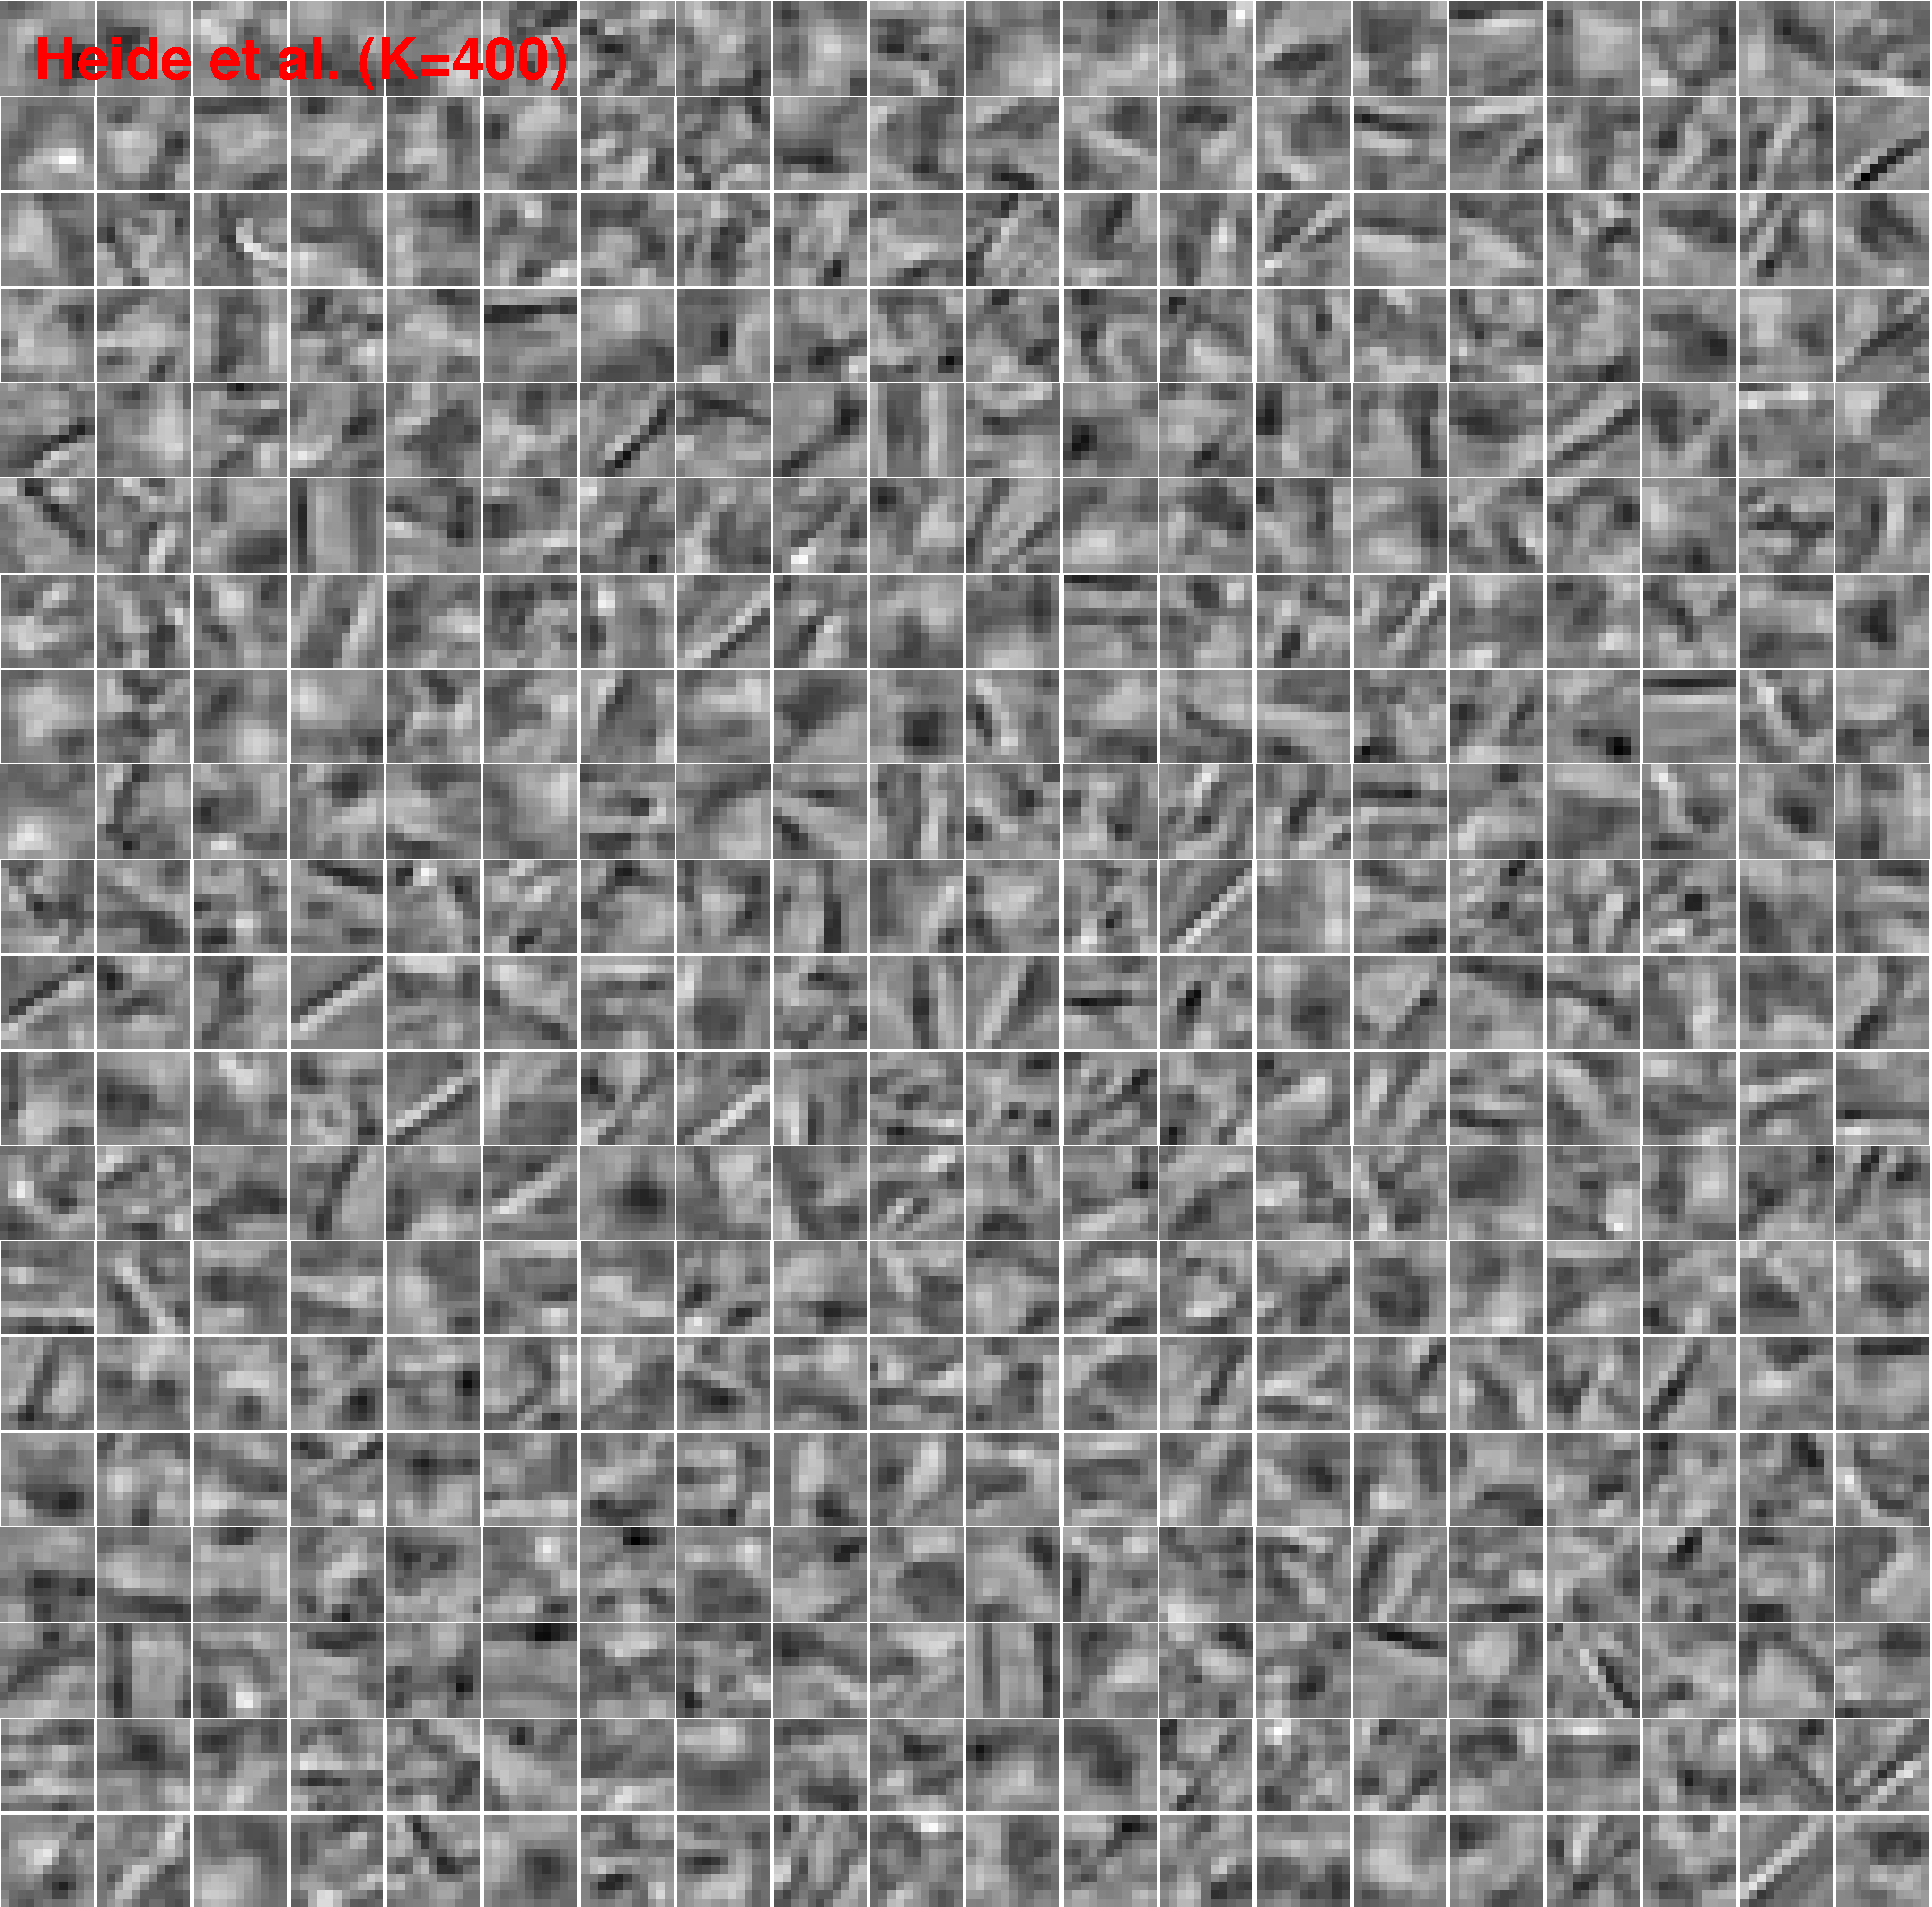
\includegraphics[width=1\linewidth]{figure/heide400-supple.pdf}
  \end{subfigure}
  \vspace{0.2cm}
  \begin{subfigure}{0.5\textwidth}
  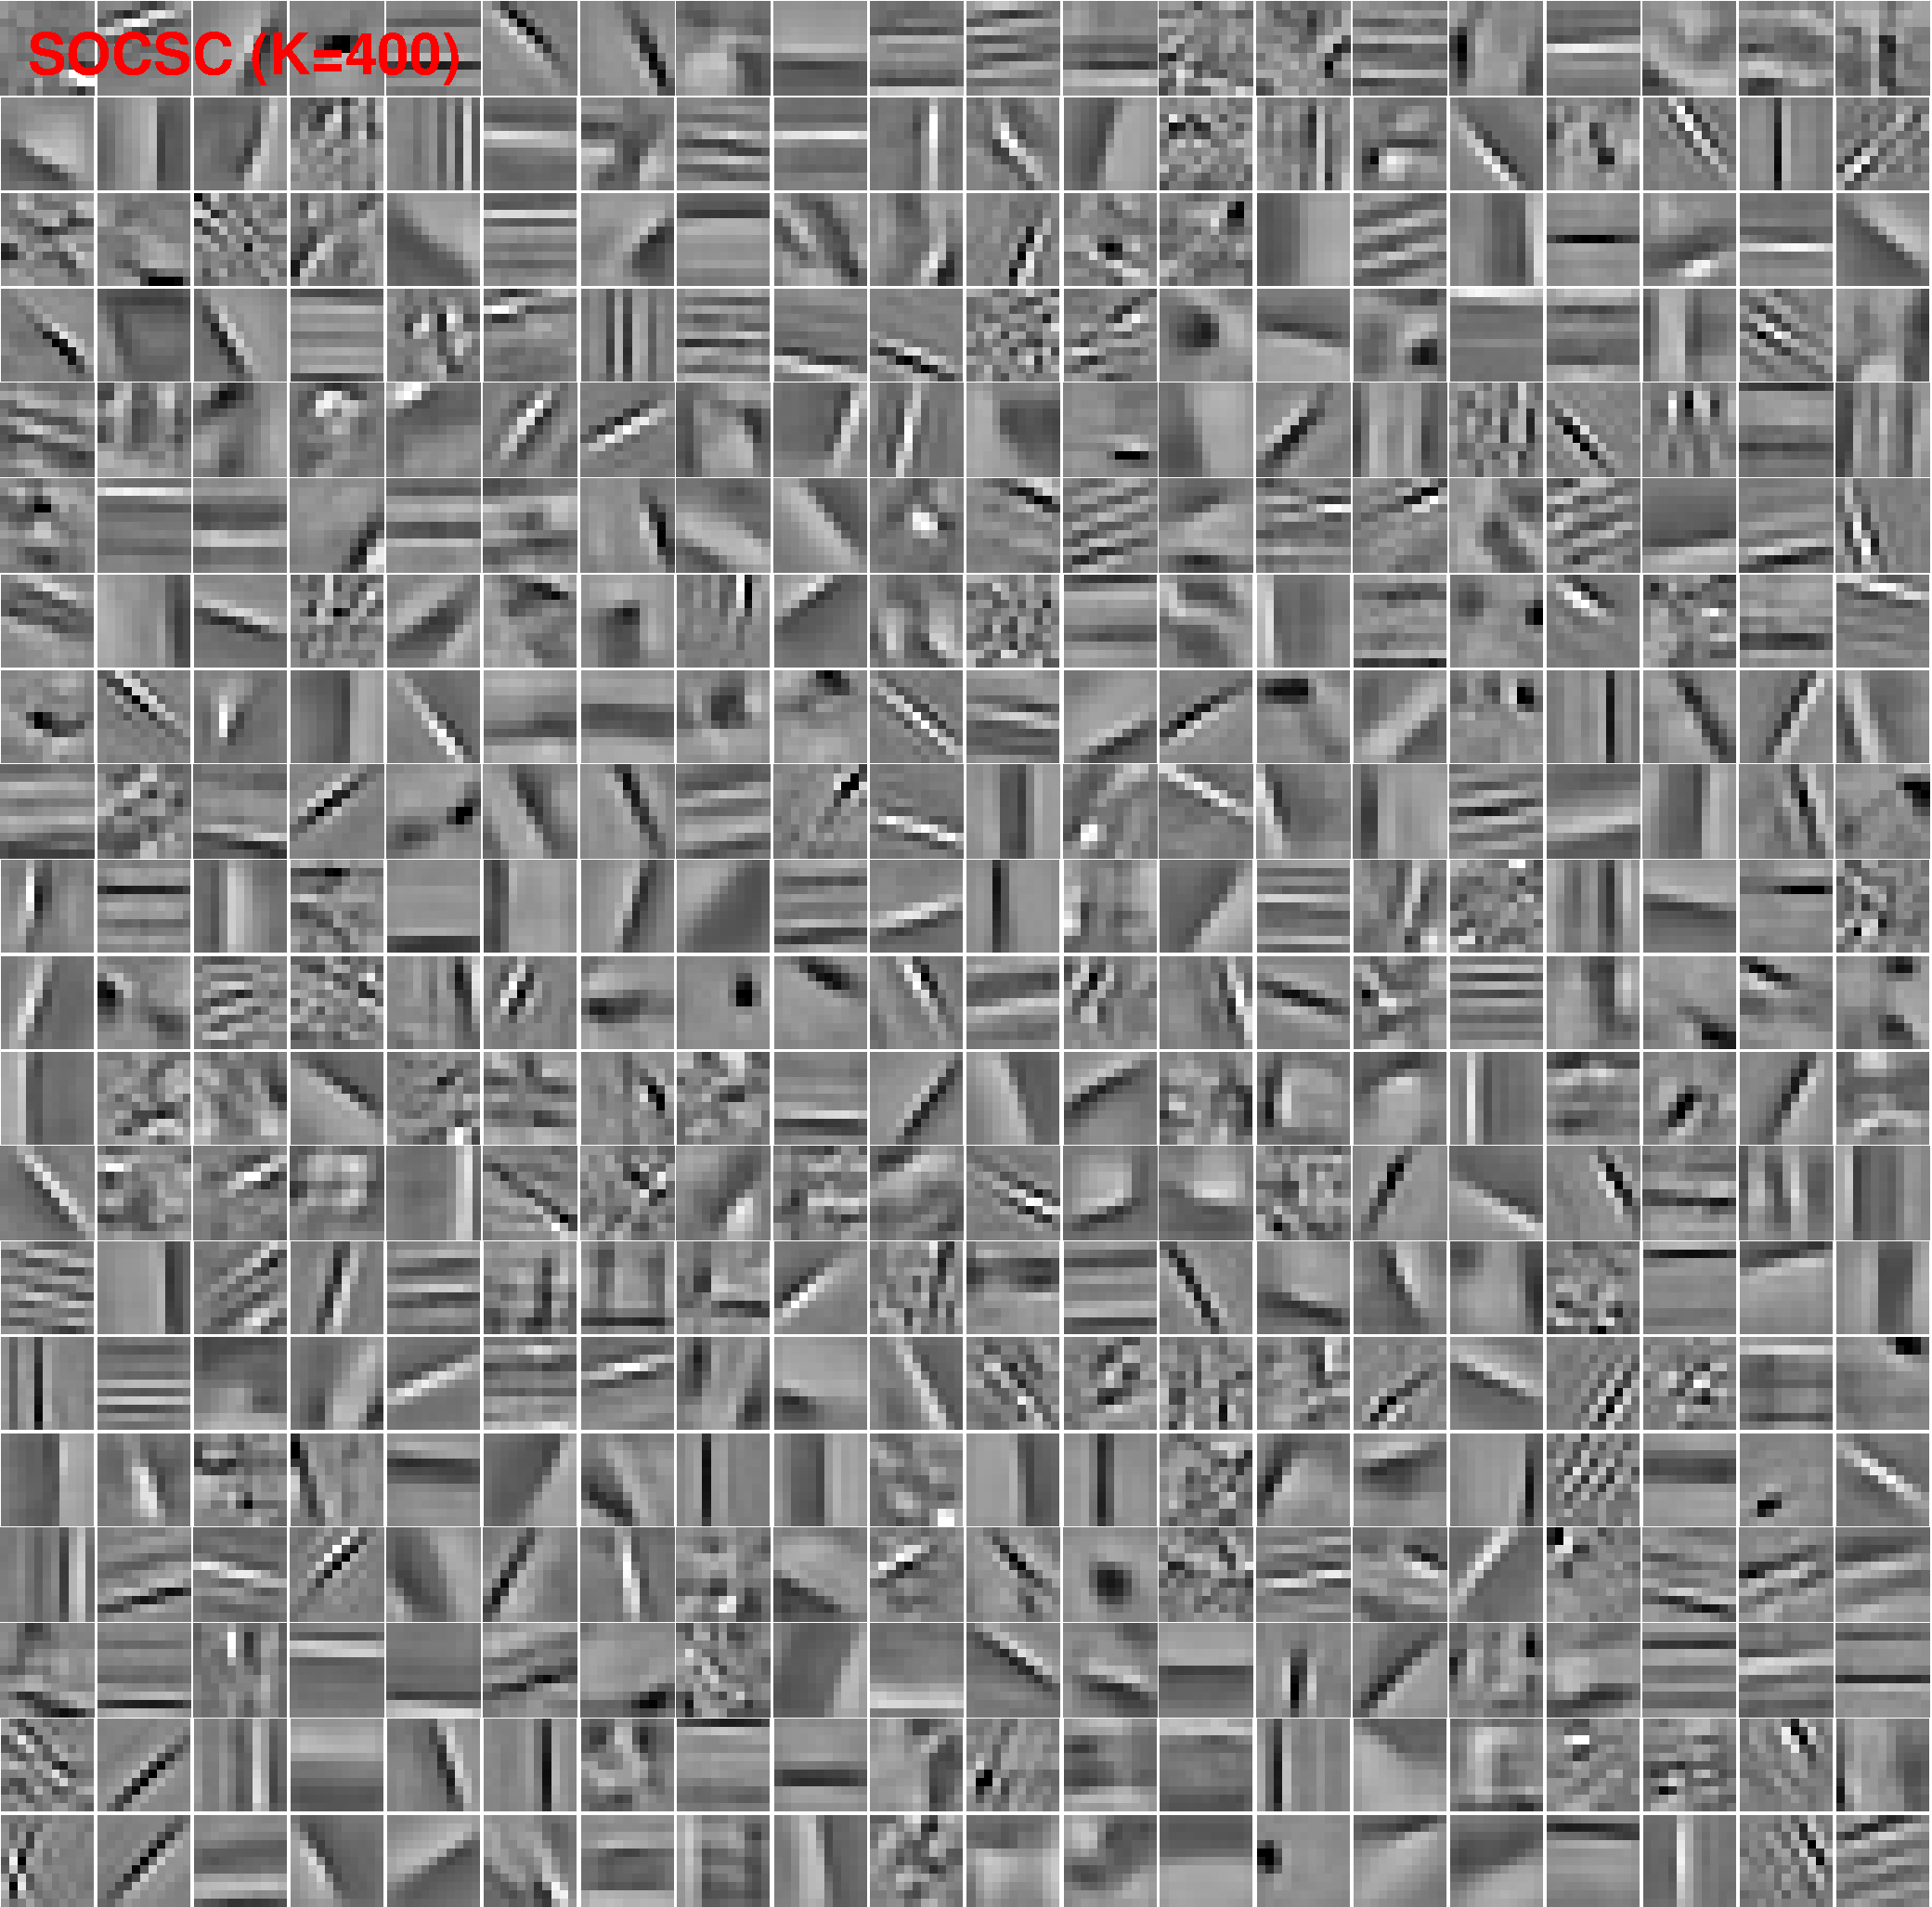
\includegraphics[width=1\linewidth]{figure/online400-supple.pdf}
  \end{subfigure}
  \vspace{0.2cm}

    \resizebox{0.8\linewidth}{!}{
        \begin{tabular}{|c||c|c|c|c|c|c|c|c|c|c|}
            \cline{1-11}
            Image & 1 & 2 & 3 & 4 & 5 & 6 & 7 & 8 & 9 & 10 \\
            \hline
            PSNR~[10] & 29.60 & 28.11 & 29.47 & 28.98 & 28.79 & 29.21 & 28.03  & 29.31 & 27.42 & 30.52 \\
            \hline
            PSNR ours & \textbf{30.24} & \textbf{28.34} & \textbf{29.95}  & \textbf{30.30} & \textbf{29.43} & \textbf{29.96} & \textbf{28.24} & \textbf{30.57} & \textbf{27.72} & \textbf{31.67} \\
            \hline
        \end{tabular} }
  \caption{ Visual and numerical comparisons between the learned over-complete dictionaries by batch-mode algorithm and by online-mode algorithm. Top: Over-complete dictionary learned by batch CSC model on small dataset, and proposed online CSC model (SOCSC) on large dataset. Bottom: Respective reconstruction quality for these two over-complete dictionaries applied for image inpainting.}
  \label{fig:overCompleteDic-dataset}
\end{figure*}

In this section, we first show the improved sparse representation of the natural images with over-complete dictionaries ($K=400$) over under-complete ones ($K=100$). The numerical comparisons of number of non-zero elements and its corresponding reconstruction PSNR for various images are shown in Fig.~\ref{fig:overVSunder}. Here, we define the non-zero elements as the codes whose coefficient is no less than $0.1$. We could observe that at all times, using over-complete dictionary leads to a sparser representation of the images, roughly $8\%-10\%$ reduction on the non-zero elements. Meanwhile, it achieves dramatically improved reconstruction quality, over $1$ dB on average.

We then verify the importance of a large dataset when learning the over-complete dictionary. in Fig.~\ref{fig:overCompleteDic-dataset}, we show a visual and quantitative comparisons between the over-complete dictionaries respectively learned by batch-mode algorithm on small dataset (the fruit dataset) and online-mode algorithm on large dataset (1000 images). Most of the filters learned from small dataset have poor structures and reveal very limited representative ability. The numerical results also demonstrate that it even shows a degraded reconstruction performance compared to the under-complete dictionary. Owing to plentiful training samples, our over-complete dictionary not only shows visually decent structures and more representative image features, but also leads to a significant improvement on image reconstruction. Based on all experimental results, it implies that the number of filters and number of training samples are both essential in the CSC model, therefore, the proposed algorithm has prominent advantages over the existing approaches.

\end{document}



% --- DO NOT DELETE ---
% Local Variables:
% mode: latex
% mode: flyspell
% mode: TeX-PDF
% End:

